\documentclass[12pt, letterpaper]{article}

%% Load packages -- build from the paper/ directory:
%%   cd paper && pdflatex main.tex
%% or set TEXINPUTS if building from repo root.
% packages.tex
\usepackage{amsmath, amssymb, amsthm}
\usepackage{graphicx}
\usepackage[
    hidelinks,
    pdftitle={A Discrete Causal Lattice Foundation for Physics},
    pdfauthor={Jack Menendez},
    pdfsubject={Discrete quantum gravity, octahedral lattice, A=1 framework},
    pdfkeywords={causal lattice, discrete spacetime, quantum gravity, octahedral, path counting}
]{hyperref}
\usepackage{booktabs}
\usepackage{array}
\usepackage{geometry}
\usepackage{adjustbox}
\usepackage{setspace}
\usepackage{caption}
\usepackage{subcaption}
\onehalfspacing

% commands.tex -- mathematical shorthand for the A=1 framework

% Theorem environments
\newtheorem{theorem}{Theorem}[section]
\newtheorem{lemma}[theorem]{Lemma}
\newtheorem{corollary}[theorem]{Corollary}

% The primal 3D topology
\newcommand{\Tdiamond}{\mathcal{T}_\diamond^3}

% Unity constraint
\newcommand{\unity}{\mathcal{A}=1}

% Phase rotor
\newcommand{\phirotor}{\phi_{\mathrm{rot}}}

% Hop probability
\newcommand{\phop}{p_{\mathrm{hop}}}

% Clock density
\newcommand{\clockdensity}{\rho_{\mathrm{clock}}}

% Path count function P(N, a, b, c)
\newcommand{\pathcount}[4]{P(#1,\,#2,\,#3,\,#4)}

% Tick operator
\newcommand{\tickop}{\hat{T}}

% Causal cone at time N
\newcommand{\causalcone}[1]{\mathcal{C}(#1)}


%% Page geometry (also set here as fallback in case packages.tex path fails)
\geometry{top=1in, bottom=1in, left=1in, right=1in}

\title{Geometry First:\\
       Quantum Mechanics, Gravity, and the Origin of the Standard Model\\
       from a Single Conservation Law%
       \thanks{Version 1.0.
       \href{https://doi.org/10.5281/zenodo.NNNNNNNN}%
            {DOI: 10.5281/zenodo.NNNNNNNN}.
       \href{https://github.com/JackDMenendez/discrete-causal-lattice}%
            {GitHub: JackDMenendez/discrete-causal-lattice}.
       Paper~I of the A=1 Discrete Causal Lattice series; companion
       papers in preparation address the Standard Model gauge
       derivation, the Farey-sequence mass spectrum (and its
       Veneziano-amplitude limiting case), plasma and
       gradient-ionization phenomenology, the proton-interior
       structure, and quantum measurement theory.}}
\author{Jack Menendez\\
        \small Eugene, OR\\
        \small ORCID: \href{https://orcid.org/0009-0003-1166-307X}{0009-0003-1166-307X}\\
        \small \href{mailto:jackdmenendez@gmail.com}{jackdmenendez@gmail.com}}
\date{\today}

\begin{document}

\maketitle

\noindent\textbf{License.}  Paper text and figures: Creative Commons
Attribution 4.0 (CC BY 4.0).  Source code in the companion
repository: MIT License.

\medskip
\noindent\textbf{Data availability.}  All numerical experiments,
data files, and the LaTeX source for this paper are publicly
available at
\href{https://github.com/JackDMenendez/discrete-causal-lattice}%
     {\texttt{github.com/JackDMenendez/discrete-causal-lattice}}.
The exact commit corresponding to this release is the v1.0 tag,
archived at
\href{https://doi.org/10.5281/zenodo.NNNNNNNN}%
     {\texttt{doi:10.5281/zenodo.NNNNNNNN}}.
A compact reproducibility quickstart, including a 10-line minimal
verification snippet, is in
Appendix~\ref{sec:reproducibility}.

\medskip
\noindent\textbf{Keywords.}  discrete spacetime; bipartite causal
lattice; single conservation law; emergent quantum mechanics;
clock-fluid gravity; Arnold-tongue quantization; induced gauge
action; lattice birefringence.

\begin{abstract}
    % ============================================================
% abstract.tex
% STATUS: STUB - populate after all sections are drafted
% ============================================================

% Key claims to address in the abstract:
% 1. The A=1 unity constraint on a 3D octahedral lattice
% 2. Per-particle tick counters and the clock-density gravity mechanism
% 3. Genuine discrete interference (no continuous Huygens formula)
% 4. The observer-as-clock formalization of the measurement problem
% 5. At least one falsifiable numerical prediction

\textbf{[STUB]} The abstract will summarize the A=1 framework applied to a
three-dimensional octahedral causal lattice $\mathcal{T}_\diamond^3$, in which
every particle carries an independent tick counter and physics emerges from the
combinatorial scheduling of those counters. Gravity arises as a clock-density
gradient rather than spacetime curvature. A falsifiable prediction concerning
discrete path-count deviations from the continuous $1/r^2$ law is derived and
proposed for experimental verification.

\end{abstract}

\bigskip
\noindent\textbf{Release notes for v1.0 (since v0.98-RC).}
v1.0 closes the release-candidate cycle.  The principal additions
since v0.98-RC are:

\begin{itemize}
\item Three new audit-table rows (Table~\ref{tab:audit}):
  long-horizon escape mechanism (\texttt{exp\_12c}, \texttt{PART});
  lock-in resonance grid-independence
  (\texttt{exp\_12d\_tight} + \texttt{exp\_12d\_outlier\_trace},
  \texttt{PART}) --- cross-grid validation of \texttt{exp\_12}'s
  4-sig-fig PASS across $\{65, 81, 97, 113\}^3$; and the Standard
  Model gauge-group conjecture as a precise Lie-algebra equality
  (\texttt{STUB}).
\item A Gleason-uniqueness subsubsection in the Born-rule
  discussion (§\ref{subsubsec:born_gleason}), addressing the
  necessity question for the $|\psi|^2$ measure that the
  v0.98-RC text only handled with a sufficiency argument.
\item An explicit metric-tensor formula in the gravity section
  (§\ref{subsec:metric_from_rho}), identifying $g_{\mu\nu}$ as a
  functional of $\rho_\text{clock}$ in the weak-field limit.
\item Refined automorphism conjecture
  (Eq.~\ref{eq:automorphism_conjecture}): now stated as an
  18-dimensional Lie-algebra equality with explicit decomposition
  into established factors ($SO(3,1) \times U(1)$ on the existing
  per-site $\mathbb{C}^2$ amplitude) and structural-extension
  factors ($SU(2)_W$ on a per-site $\mathbb{C}^2$ isospin index;
  $SU(3)$ on a per-site $\mathbb{C}^3$ colour index).  Six
  computational scaffolding scripts in \texttt{src/utilities/}
  establish each component.
\item Acknowledgements section
  (Section~\ref{sec:acknowledgements}).
\end{itemize}

\emph{Status legend used throughout.}  \texttt{PASS} = derivation
complete or experiment confirms the claim to stated precision.
\texttt{PART} = mechanism demonstrated, full quantitative match
pending; specific gaps documented in the evidence column of
Table~\ref{tab:audit}.  \texttt{STUB} = analytical result with no
numerical confirmation yet.  \texttt{FAIL} = tested and
disconfirmed.

\emph{Out-of-scope for v1.0.}  The Standard Model gauge-group
derivation, the Farey-sequence mass spectrum, the proton-interior
structure, plasma and gradient-ionization phenomenology, quantum
measurement theory, and the combinatorial foundations of
continuum physics (Hilbert's 6th problem) are explicit subjects
of follow-on papers; the present paper establishes the
foundational framework on which they build.

A detailed change log is in
\texttt{release\_notes/v1.0.md} in the project repository.
Earlier versions remain available at the Zenodo deposit's prior
DOIs.

\newpage
\tableofcontents
\newpage

%% ============================================================
%% PART I: FOUNDATIONS
%% ============================================================
\section{Introduction}
% ============================================================
% introduction.tex
% ============================================================

Quantum mechanics is the most precisely verified theory in the history
of science.
It answers, with extraordinary accuracy, every question about how particles
behave: what energies they occupy, how they scatter, how they interfere,
how they decay.
But it is structurally silent on a different class of questions --- why
its own axioms hold.

Why are atomic spectra discrete rather than continuous?
The Schr\"odinger equation produces discrete eigenvalues given the right
boundary conditions, but the boundary conditions are loaded into the
formalism before the calculation begins.
Why is the Born rule $|\psi|^2 = \text{probability}$ true?
It is a postulate --- von Neumann's measurement axiom --- not a derivation.
Why do the Dirac gamma matrices have the algebraic structure they do?
Dirac constructed them to satisfy his requirements; they were
not derived from anything geometrically prior.
Why is the gauge group of the Standard Model $\mathrm{SU}(3)\times
\mathrm{SU}(2)\times\mathrm{U}(1)$ and not some other group?
The Standard Model takes its gauge content as given.

These are not criticisms of quantum mechanics.
They are a precise statement of what it is silent about, and that silence
has been known since at least von Neumann~\cite{vonneumann1932} and is
uncontroversial.
A framework that answered these questions would not replace quantum mechanics;
it would explain it.

\medskip

This paper proposes such a framework.
We show that all four questions have geometric answers, and that all four
answers follow from a single conservation law:

\begin{center}
\textbf{Conservation of probability --- the axiom $\mathcal{A}=1$.}
\end{center}

On a bipartite three-dimensional causal lattice $\mathcal{T}_\diamond^3$,
each particle is a \emph{causal session}: an independent phase rotor
carrying amplitude $(\psi_R, \psi_L)$ on the two chirally-opposite
sublattices, subject to $|\psi_R|^2 + |\psi_L|^2 = 1$ at every tick.
No Hamiltonian, no Hilbert space, and no measurement postulate are
assumed.

The four answers:
\begin{enumerate}
\item \textbf{Quantization is an attractor, not a boundary condition.}
    The discrete mass spectrum arises from Arnold tongue frequency-locking
    between the particle's internal Zitterbewegung frequency and the vacuum
    carrier.
    Any nearby frequency is dynamically pulled into the nearest rational
    resonance basin.
    Discreteness is self-organising, not postulated.

\item \textbf{The Born rule follows from $\mathcal{A}=1$.}
    Probability is amplitude squared because amplitude is the only
    physical quantity on the lattice and $\mathcal{A}=1$ is the
    conservation law that governs it.
    The Born rule is not a measurement axiom; it is a conservation theorem.

\item \textbf{The Dirac gamma matrices encode lattice geometry.}
    The bipartite RGB/CMY sublattice structure \emph{is} the two-component
    Dirac spinor.
    In the continuum limit $a\to 0$, the tick rule converges to the
    Dirac equation $(i\gamma^\mu\partial_\mu - m)\psi = 0$, with the
    gamma matrices identified as the geometric encoding of three pairs
    of antiparallel basis vectors.
    The Clifford algebra $\{\gamma^\mu,\gamma^\nu\} = 2g^{\mu\nu}$ holds
    because the basis vectors form a tight frame --- a geometric theorem,
    not an algebraic postulate.

\item \textbf{Photon emission is a conservation-law necessity.}
    The Coulomb interaction is a probability \emph{source} --- it injects
    amplitude into the electron session from outside.
    $\mathcal{A}=1$ cannot accommodate this within a single session;
    it mandates creation of a new photon session at orbital lock-in.
    Emission, recoil, and energy conservation all follow from
    $\mathcal{A}=1$ alone.

\item \textbf{Gravity is refraction, not curvature.}
    Every causal session carries an independent tick counter.
    The local density of these clocks --- the session density weighted by
    probability --- is the gravitational field.
    Causal paths refract toward regions of higher clock density by the
    same mechanism as Fermat's principle in optics: amplitude hops
    preferentially toward nodes where the phase cost is lower.
    No curved geometry is required.
    Gravitational time dilation is scheduler load: a clock near a mass
    processes more causal events per external tick and therefore runs
    slow.
    The equivalence principle is structural: both gravitational and
    inertial mass arise from the same phase-mismatch parameter $\omega$,
    so their equality requires no explanation.
    The event horizon is scheduler saturation --- a computational
    deadlock at the Planck density ceiling $\rho_\text{max} =
    \ell_P^{-3}$ --- with no singularity, and Hawking radiation as
    stochastic queue-drop.
    In the continuum limit the clock fluid equations reduce to the
    Einstein field equations; at finite lattice spacing they carry
    discrete corrections to the $1/r^2$ law that are computable and
    falsifiable.
\end{enumerate}

\medskip

A further result, which we consider the deepest, concerns the nature of
bound states.
The standard treatment of hydrogen places the proton as a fixed external
potential $V(r) = -e^2/r$ and solves for the electron's eigenstates.
This is not merely an approximation --- it is the wrong physical picture.

A static Coulomb potential is insufficient to produce stable quantised
orbits from the lattice dynamics alone.
The proton must be represented as an active session --- a phase rotor
participating in the joint $\mathcal{A}=1$ accounting every tick ---
for the electron to explore the well and lock onto resonant orbits
spontaneously.
Hydrogen is not an electron in a field.
It is \emph{two sessions finding a joint Arnold tongue attractor.}

This distinction has directly observable consequences.
In a static well the electron collapses to the potential minimum regardless
of initial momentum; the basin of attraction around the Bohr orbit has
zero width (\texttt{exp\_11} $n=2$: flat landscape across all
$k$-values tested).
With an active proton session, the proton's Zitterbewegung continuously
breaks the spherical symmetry of the potential, providing the stochastic
perturbation that drives the electron into the resonance basin;
the Bohr orbital wavevector is recovered to four significant figures
with no parameter tuning (\texttt{exp\_12}).
The basin of attraction is finite and self-correcting --- the orbit is
stable not because we initialised it exactly, but because the two-session
dynamics continuously restores it.

Photon emission then follows as a three-session event: the joint
proton-electron resonance transitions to a lower Arnold tongue, the
displaced amplitude is absorbed by a new photon session, and the proton
adjusts to the new joint configuration.
None of this requires a separately postulated transition rate.

\medskip

\paragraph{Relation to prior discrete spacetime programmes.}
The $\Tdiamond$ framework belongs to a tradition of discrete spacetime
proposals that includes causal set theory~\cite{bombelli1987},
'T~Hooft's cellular automaton interpretation~\cite{thooft2016},
Wolfram's computational universe~\cite{wolfram2002}, and Zuse's
Rechnender Raum~\cite{zuse1969}.
It differs from these in the precision of its structural claims and the
number of falsifiable numerical predictions it makes without free
parameters.
The frame condition $\sum_\text{RGB}\mathbf{v}_i\mathbf{v}_j^T = 3\delta_{ij}$
is not a tuning choice; it is a geometric identity of the RGB basis vectors
that forces the Clifford algebra and the isotropic dispersion relation
simultaneously.
The lattice does not approximate known physics --- it derives it from
a single conservation law and a single geometric substrate.

\paragraph{Organisation of the paper.}
Section~\ref{sec:substrate} defines the $\Tdiamond$ lattice, its
bipartite structure, and the calibration of physical units.
Section~\ref{sec:causal_sessions} introduces causal sessions and the
phase rotor.
Sections~\ref{sec:tick_scheduler}--\ref{sec:kinematics} derive
momentum, force, and the Dirac equation from the tick rule.
Sections~\ref{sec:gravity}--\ref{sec:vacuum_twist} treat gravity
and electromagnetism as distinct phase geometries.
Sections~\ref{sec:interference}--\ref{sec:observer} cover interference,
decoherence, and the observer.
Sections~\ref{sec:predictions}--\ref{sec:hydrogen} present the
falsifiable predictions and the hydrogen results.
Section~\ref{sec:conclusion} states what has been established and
what remains open.


\section{The Octahedral Substrate \texorpdfstring{($\Tdiamond$)}{(T\_diamond\textasciicircum 3)}}
% ============================================================
% octahedral_substrate.tex
% STATUS: STUB
% Corresponds to: src/core/OctahedralLattice.py
% Experiment: exp_00_causal_cone.py
% ============================================================

% Topics to cover:
% - Why octahedral? 6 neighbors, coordination number, isotropy argument
% - Node definition: an event, not a location
% - Edge definition: causal adjacency in 3D
%   - The 6 principal directions: {+x,-x,+y,-y,+z,-z}
% - The 3D causal cone: expanding octahedron, not a sphere
% - Path counting on the octahedral lattice
%   - Exact integer count for N hops to node (a,b,c)
%   - Convergence to Gaussian (CLT bridge)
%   - Deviations from Gaussian at small N (the falsifiable regime)
% - Calibration: mapping node separation to physical units
%   - Planck scale calibration
%   - Alternative calibrations (Bohr radius, Compton wavelength)
% - Comparison to causal set theory (Sorkin, Bombelli)
%   - What is the same, what is distinct

\textbf{[STUB]}


\section{Causal Sessions and the Phase Oscillator}
% ============================================================
% causal_sessions.tex
% STATUS: STUB
% Corresponds to: src/core/CausalSession.py, src/core/PhaseRotor.py
% Experiment: exp_01_inertia.py
% ============================================================

% OPEN QUESTION (from exp_01 results):
% In the current tick() implementation, higher omega causes FASTER propagation
% given the same phase gradient, because omega amplifies the phase-alignment
% weighting. True inertial behavior requires heavier particles to resist
% changes in velocity -- omega should damp the phase-alignment response,
% not amplify it. The correct formulation needs further work.
% Candidate fix: weight emission by 1/(omega * phase_alignment) so that
% high-frequency packets are less responsive to the gradient per tick.
% This is the key open theoretical question for Section 3.


% - The CausalSession: a particle as a persistent probability flux
% - The PhaseRotor: U(1) internal clock
%   - omega as instruction frequency (mass)
%   - Phase gradient as momentum
% - The hop probability distribution
%   - At rest: 1/6 to each neighbor, probability of staying put
%   - In motion: asymmetric distribution encoding velocity
%   - The temperature analogy for the stay-put probability
% - Compact support: probability strictly zero outside causal cone
% - Inertia as phase-gradient persistence (U(1) stability)
% - Mass as instruction overhead: F = ma as state-update cost

\textbf{[STUB]}


%% ============================================================
%% PART II: DYNAMICS
%% ============================================================
\section{The Tick Scheduler}
% ============================================================
% tick_scheduler.tex
% Section 4: The Tick Scheduler
% Corresponds to: src/core/TickScheduler.py
% Experiments: exp_05_observer_clock.py, exp_07_clock_conservation.py
% ============================================================

\label{sec:scheduler}

The previous section defined a single causal session: a U(1) phase
oscillator on the $\Tdiamond$ lattice with its own tick counter, evolving
under the bipartite tick rule and obeying the $\unity$ constraint at every
tick.
A real physical situation is rarely one session.
Atoms are at least two; molecules many; macroscopic bodies astronomically
many.
The \emph{tick scheduler} is the architectural component that turns a
collection of independent sessions into the dynamics of an interacting
universe.

The scheduler is conceptually small.
It maintains a list of registered sessions, advances each session by one
tick in some order, and applies an interaction step that exchanges phase
between sessions whose probability supports overlap.
That is the whole machine.
The richness of the framework comes from what follows from those two
operations.
This section sets out the formal apparatus.
The phenomenological consequences --- measurement
(Section~\ref{sec:observer}), gravity
(Section~\ref{sec:gravity}), spontaneous emission
(Section~\ref{subsec:emission}) --- are derived from the scheduler in
later sections.

% ── 4.1 The Macro-Tick ────────────────────────────────────────────────────────
\subsection{The Macro-Tick}
\label{subsec:macro_tick}

A \emph{macro-tick} is one cycle of the scheduler.
For a scheduler with $n$ registered sessions
$\{\mathcal{S}_1, \ldots, \mathcal{S}_n\}$, one macro-tick consists of
three steps:

\begin{enumerate}
    \item \textbf{Order.}  Determine a processing order
    $\sigma \in S_n$ over the sessions according to the active shuffle
    scheme.
    \item \textbf{Tick.}  For each $i$ in the order $\sigma$, advance
    $\mathcal{S}_i$ by one bipartite tick (Section~\ref{sec:phase}) and
    increment its tick counter.  Each session enforces $\unity$
    individually after its own tick.
    \item \textbf{Couple.}  Apply the pairwise phase-exchange step
    (Section~\ref{subsec:binding}) at every node where two sessions have
    significant probability support.  Apply any registered three-session
    couplings (Section~\ref{subsec:emission_coupling}).
\end{enumerate}

The decomposition into \emph{tick} and \emph{couple} is essential.
Each session is independently norm-preserving during the tick step ---
this is what makes the U(1) group structure of
Section~\ref{subsec:phase_oscillator} survive at the multi-session level.
The couple step then redistributes \emph{phase} between sessions at
shared nodes without moving probability across them.
$\unity$ is preserved per session through both steps; what is shared is
the coherent structure of the wavefunction, not the probability mass.

In code, the macro-tick is the \texttt{TickScheduler.advance} method.
The full state of the universe at macro-tick $n$ is the tuple
$(\{\mathcal{S}_i\}, \sigma_n, n)$: the sessions, the ordering used at
this step, and the global cycle count.

% ── 4.2 The Combinatorial Clock Space ─────────────────────────────────────────
\subsection{The Combinatorial Clock Space}
\label{subsec:clock_space}

The scheduler's state space is the set of orderings of its registered
clocks.
For $n$ sessions this is the symmetric group $S_n$, of size
\begin{equation}
    |\Omega_n| = n!.
    \label{eq:state_space_factorial}
\end{equation}
This factorial growth is the algebraic root of the framework's
treatment of time.
It will appear again as the entropy of an observer interaction
(Section~\ref{subsec:irreversibility}), as the load on a region near
mass concentrations (Section~\ref{subsec:density_dilation}), and as the
combinatorial source of the second law
(Section~\ref{subsec:arrow_of_time}).

\paragraph{Shuffle schemes as experimental variables.}
The framework does not fix a single ordering rule.
Four schemes are implemented:

\begin{itemize}
    \item \textsc{Sequential}: process sessions in registration order.
    \item \textsc{Random}: uniform random shuffle each macro-tick.
    \item \textsc{Priority}: lowest tick counter first.
    \item \textsc{Clock-density}: highest local
    $\clockdensity$ first.
\end{itemize}

If the framework is correct as a model of physics, the bulk
phenomenology --- conserved probability, the Dirac equation in the
continuum limit, gravitational attraction --- should be invariant under
the choice of scheme.
Different schemes correspond to different choices of simultaneity for the
discrete substrate, in close analogy to choices of foliation in general
relativity.
A discrete \emph{Lorentz invariance} is the prediction that the
choice does not matter for any observable bulk quantity.

\paragraph{Numerical verification (\texttt{exp\_05}).}
The conserved-probability check is straightforward and was performed in
\texttt{exp\_05}.
Across all three implemented schemes
(\textsc{sequential}, \textsc{random}, \textsc{priority}) and across
session counts $n = 1, 2, 3, \ldots, 6$, the total probability satisfies
$|\sum_i \rho_i - n| < 10^{-15}$ at every macro-tick --- machine precision
conservation independent of ordering.
The deeper question --- whether two observers using different shuffle
schemes can disagree on a measurement outcome --- is treated in
Section~\ref{sec:observer}.
The answer is no: the only quantities that depend on the ordering are
those that depend on \emph{which} cone perturbed which, not on the
final probability distribution.

% ── 4.3 Pairwise Coupling and the Binding Dial ────────────────────────────────
\subsection{Pairwise Coupling and the Binding Dial}
\label{subsec:binding}

Two sessions registered in the same scheduler are not, by themselves,
coupled.
They share a lattice but evolve independently.
Coupling enters through the third step of the macro-tick: at any node
$\mathbf{x}$ where two sessions $\mathcal{S}_i$ and $\mathcal{S}_j$ both
have significant amplitude (above a threshold $\sim 10^{-4}$), their
phases are partially exchanged.

The mechanism is a U(1) rotation in the orbital plane of phase
$\phi_i = \arg(\psi_R^{(i)})$ at each shared node:
\begin{align}
    \phi_i &\to \phi_i + c_{ij}\,(\phi_j - \phi_i), \\
    \phi_j &\to \phi_j + c_{ij}\,(\phi_i - \phi_j),
    \label{eq:phase_mix}
\end{align}
where $c_{ij} \in [0, 1]$ is the binding strength registered for the
pair.
Both spinor components are rotated by the same phase
($\unity$ does not mix $\psi_R$ with $\psi_L$ here), and each session is
re-normalised after the rotation.

The single parameter $c_{ij}$ encodes the entire spectrum of two-session
relationships:

\medskip
\begin{center}
\begin{tabular}{ll}
\hline
$c_{ij}$ & Physical regime \\
\hline
$0$       & Free particles --- no interaction \\
$\sim 0.1$ & Weak --- observer / decoherence regime \\
$\sim 0.5$ & Atomic binding --- joint Arnold tongue \\
$\sim 0.9$ & Strong binding --- composite particle \\
$1$       & Phase lock --- sessions move as a single unit \\
\hline
\end{tabular}
\end{center}
\medskip

The same algebraic step thus produces, in different parameter regimes,
the observer effect of Section~\ref{sec:observer}, the joint hydrogen
resonance of Section~\ref{subsec:exp12}, and the bound-state binding
that defines composite particles.
A neutral composite (a neutron, a hydrogen atom seen from far away) is
two or more sessions with $c \to 1$ \emph{and} opposite RGB/CMY
imbalance: their phase gradients cancel, narrowing the effective causal
cone of the composite below those of its constituents.
This cone narrowing is the lattice mechanism for why neutral matter
behaves more classically than its charged constituents.

% ── 4.4 Three-Session Coupling and Emission ───────────────────────────────────
\subsection{Three-Session Coupling and Emission}
\label{subsec:emission_coupling}

Some interactions cannot be reduced to pairwise phase exchange.
The clearest example is spontaneous emission, which we showed in
Section~\ref{subsec:emission} to be a three-session event: the joint
electron--proton resonance jumps to a lower Arnold tongue, and a third
session (the photon) is created to absorb the displaced amplitude under
$\unity$.
The scheduler accommodates this by maintaining an explicit list of
\emph{emission triplets} $(\mathcal{S}_e, \mathcal{S}_\gamma,
\mathcal{S}_p, r)$, where $r$ is the per-tick drain rate.

The drain step is engineered to respect $\unity$ exactly.
At each macro-tick the electron's tangential phase gradient
$\nabla_\perp\phi_e$ (the radial component is preserved so the Coulomb
attraction continues to act) is rotated by $-r\,k_\text{tang}\cdot s$,
where $s$ is the arc-length coordinate along the orbital plane and
$k_\text{tang}$ is the current orbital wavevector.
The conjugate rotation is applied to the photon, transferring orbital
angular momentum from electron to photon while leaving the per-session
probability density --- and therefore $\unity$ --- untouched.
The \emph{appearance} of dissipation comes from the subsequent
re-normalisation step, which sees a redistributed phase structure and
adjusts the spinor components accordingly.

The three-session coupling is the clearest demonstration that the
scheduler is more than a clock-shuffler.
It is a mechanism that decides, at each tick, which combinations of
sessions are interacting and how.
Pairwise binding handles two-session phenomena; emission triplets
handle three-session events; further $n$-session generalisations
(electroweak vertices, hadronic decays) follow the same pattern of
explicit registration with an $\unity$-preserving update rule.

% ── 4.5 Clock Density and Time Dilation ───────────────────────────────────────
\subsection{Clock Density and Time Dilation}
\label{subsec:density_dilation}

The pairwise step of the macro-tick scales with the number of session
overlaps.
For $n$ sessions with significant pairwise support there are at most
$\binom{n}{2}$ pairs to evaluate; for sessions whose probability supports
all share a common node, every pair contributes.
The scheduler is therefore not a constant-cost machine.
Regions of the lattice where many sessions overlap impose more
bookkeeping per macro-tick than regions where sessions are isolated.

This is the lattice substrate for gravitational time dilation.
A region of high clock density $\clockdensity$ runs more couplings per
macro-tick.
A session embedded in that region executes its own tick rule
unchanged --- but each macro-tick it is processed alongside more
neighbours, with more phase exchanges to settle.
From the perspective of a distant observer, who sees only the global
macro-tick count $n$, the local session has accumulated fewer
``personal'' tick advances per global macro-tick: its clock runs slow.

The continuum-limit derivation of this picture --- with the explicit
identification $\nabla\phi_\text{Newton} \leftrightarrow$ macro-tick
imbalance and the recovery of the Schwarzschild time dilation factor
--- is given in Section~\ref{sec:gravity}.
The point here is architectural: time dilation is not added by hand
through a metric.
It is the unavoidable consequence of running a scheduler whose
per-macro-tick cost is proportional to the local session density.

% ── 4.6 Queue Saturation and the Event Horizon ────────────────────────────────
\subsection{Queue Saturation and the Event Horizon}
\label{subsec:saturation}

The scheduler can register at most one session per Planck volume.
Each session occupies a U(1) oscillator at a node, and the lattice
provides a finite number of nodes per unit volume.
The maximum clock density is therefore
\begin{equation}
    \clockdensity^\text{max} = \ell_P^{-3}
        \approx 2.37 \times 10^{104}\ \text{clocks/m}^3,
    \label{eq:rho_max_scheduler}
\end{equation}
the same bound that appears in Section~\ref{subsec:black_holes}.
At this density the scheduler queue is saturated: every available node
is bound to a session, and the next registration cannot proceed.

Saturation is the lattice definition of an event horizon.
From the outside, sessions in the saturated region cannot accept new
clock registrations and so cannot accept new information; the local
tick rate falls to zero relative to the global macro-tick.
This is not a coordinate singularity but a computational deadlock,
strictly bounded above.
There is no infinite curvature inside the horizon because there is no
infinite density: the substrate runs out of nodes before the divergence
can occur.

\paragraph{Hawking radiation as queue-drop.}
A scheduler that has reached saturation but receives further
registration attempts must do something.
The architecturally simplest response is to occasionally drop the
oldest registered session at the boundary, freeing a node for the
incoming registration.
The drop is stochastic over the boundary and proportional to the
attempted registration rate.
Each drop releases a session into the surrounding lower-density region,
where it propagates outward at $c$ along a geodesic of the clock fluid.
The thermal character of the resulting radiation --- the Hawking
spectrum --- is the thermodynamic fingerprint of a uniform-prior
boundary queue under stochastic drop, and is recovered without
trans-Planckian field modes.

\paragraph{The Hawking temperature from boundary surface gravity.}
The temperature of the queue-drop emission can be fixed to leading
order under one modelling assumption: that the saturation boundary
inherits, as an external metric quantity, the Schwarzschild surface
gravity
\begin{equation}
    \kappa = \frac{c^4}{4 G M},
    \label{eq:surface_gravity}
\end{equation}
where $M$ is the total mass enclosed by the saturated region.
This assumption is the architectural counterpart of identifying the
saturation boundary with a black-hole horizon
(Section~\ref{subsec:black_holes}); the strong-field clock-fluid
derivation that fixes the metric to Schwarzschild form is reserved
for the gravitational-continuum-limit work of
Section~\ref{sec:clock_fluid}.

A boundary with effective surface acceleration $\kappa$ supports an
Unruh-style local thermal spectrum at temperature
$T_\text{local} = \hbar\kappa/(2\pi c\,k_B)$.
Folding the gravitational redshift between the local frame and the
asymptotic observer (which, near the horizon, exactly cancels the
$1/\sqrt{1-r_s/r}$ blueshift of $T_\text{local}$) leaves the
temperature seen at infinity equal to the surface-gravity expression
itself~\cite{hawking1975}:
\begin{equation}
    T_H \;=\; \frac{\hbar\,\kappa}{2\pi\,c\,k_B}
        \;=\; \frac{\hbar\,c^3}{8\pi\,G\,M\,k_B}.
    \label{eq:hawking_T}
\end{equation}
The queue-drop rate at the saturated boundary is therefore set, up
to architectural constants of order unity, by
$\Gamma_\text{drop}\sim \kappa/(2\pi)$: the boundary releases on
average one session per $2\pi/\kappa$ of asymptotic time.

\paragraph{Honest scope of Eq.~\eqref{eq:hawking_T}.}
The lattice contribution is the architectural claim that
\emph{some} thermal emission must occur at the saturated boundary
because the scheduler cannot accept further registrations and the
queue-drop is the architecturally simplest legal response.  The
specific form $T_H = \hbar c^3/(8\pi G M k_B)$ then follows from
Eq.~\eqref{eq:surface_gravity} via the standard Unruh--horizon
relation.  The modelling assumption that fixes the numerical
prefactor is the inheritance of the Schwarzschild $\kappa$ at the
saturation boundary: a strong-field derivation of this
correspondence from the clock-fluid equations is the natural
follow-on calculation.

% ── 4.7 Architectural Irreversibility and the Arrow of Time ───────────────────
\subsection{Architectural Irreversibility and the Arrow of Time}
\label{subsec:arrow_of_time}

The scheduler has a \texttt{register\_session} method.
It does not have a \texttt{remove\_session} method, by design.

This single architectural fact is enough to derive the second law of
thermodynamics for the framework.
A measurement, in the sense of Section~\ref{sec:observer}, is the
registration of a new session that overlaps an existing one.
After the registration the state space has grown from $|\Omega_{n-1}| =
(n-1)!$ to $|\Omega_n| = n!$, an increase by a factor of $n$.
The corresponding entropy of the scheduler state space,
\begin{equation}
    S_\text{scheduler} = k_B \log |\Omega_n| = k_B \log(n!),
    \label{eq:scheduler_entropy}
\end{equation}
strictly increases with each registration, and by Stirling's
approximation grows as $S \sim k_B\,n \log n$ for large $n$.
There is no operation that can decrease $n$.
The arrow of time is not a thermodynamic approximation that becomes
exact in some statistical limit --- it is a structural feature of the
scheduler interface.

The deeper consequence, derived in Section~\ref{subsec:irreversibility},
is that what we ordinarily call the second law is the same statement as
``measurement is irreversible.''
Both follow from the absence of a clock-removal operation.
You cannot un-observe a particle for the same reason you cannot reduce
the entropy of an isolated system: the scheduler does not expose the
operation that would let you.

% ── 4.8 Falsifiable Consequences ──────────────────────────────────────────────
\subsection{Falsifiable Consequences}
\label{subsec:scheduler_predictions}

The scheduler architecture makes one prediction directly that distinguishes
it from any continuum-time formalism.

\paragraph{Minimum time-dilation quantum.}
Each registered session contributes one tick of bookkeeping per
macro-tick.
The minimum increment of gravitational time dilation between two
neighbouring regions is therefore one tick duration:
\begin{equation}
    \delta t_\text{min} = t_\text{tick},
    \label{eq:min_dilation}
\end{equation}
where $t_\text{tick}$ is the lattice tick duration in seconds.
At Planck calibration, $t_\text{tick} = t_P \approx 5.4 \times 10^{-44}$~s
and the prediction is unmeasurable.
At Compton calibration, $t_\text{tick} \approx 8 \times 10^{-21}$~s,
which is within roughly two orders of magnitude of current optical-clock
fractional sensitivity ($\sim 10^{-18}$ over millimetre baselines).
Section~\ref{sec:predictions} develops the experimental geometry that
would convert this predicted floor into a falsifiable null-result test:
if optical clocks separated by a calibrated $\Delta\phi$ in a
controlled potential gradient ever resolve a continuous distribution of
fractional offsets without a discrete cutoff, the framework is wrong.

\paragraph{Discrete corrections in queue dynamics.}
Two further structural predictions follow from queue saturation, but
their numerical form requires the gravitational continuum-limit
derivation of Section~\ref{sec:clock_fluid}.
These are: (i) a Planck-density cutoff to gravitational wave dispersion,
producing frequency-dependent gravitational-wave speeds in regions
approaching $\clockdensity^\text{max}$; and (ii) a queue-drop signature
in Hawking emission spectra at the high-frequency tail, where the
finite-lattice cutoff replaces the trans-Planckian modes of standard
treatments.
Both feed into Section~\ref{sec:predictions}.


\section{Phase Propagation and the Unity Constraint}
% ============================================================
% phase_propagation.tex
% STATUS: STUB
% Corresponds to: src/core/UnityConstraint.py
% Experiment: exp_03_interference.py
% ============================================================

\label{sec:phase}

% Topics to cover:
% - The unitary update cycle: the tick
% - Complex amplitudes at each node (not densities)
%   - Phase must survive to the summation step
%   - |psi|^2 taken AFTER summation, not before
%   - This is why interference works: signed cancellation
% - The discrete Hamiltonian as phase routing matrix
%   H(x,y,z) = omega + V(x,y,z)
% - The A=1 unity constraint
%   - Normalization after every tick
%   - Physical interpretation: probability is conserved, not created
%   - Contrast with v1.0: this must be enforced structurally, not just renormalized
% - The CLT bridge: N hops -> Gaussian -> Schrodinger equation
%   - At what N does the continuous approximation become valid?
%   - Below that N: discrete corrections exist and are calculable
% - Boundary conditions on the octahedral lattice

\textbf{[STUB]}


\section{Emergent Kinematics on the \texorpdfstring{$\Tdiamond$}{T\_diamond\textasciicircum 3} Lattice}
\section{Emergent Kinematics on the $\Tdiamond$ Lattice}
\label{sec:kinematics}

Momentum, inertia, and force are not postulated in the $\unity$ framework.
They emerge from the geometry of phase interference across the bipartite
sublattice structure.  This section derives the kinematic relations
from the Dirac tick rule and connects each result to the corresponding
numerical verification in the experiment suite.

% ── Subsection 1 ─────────────────────────────────────────────────────────────
\subsection{The Bipartite Velocity}
\label{subsec:bipartite_velocity}

A massive Dirac fermion~\cite{dirac1928} on $\Tdiamond$ carries two spinor components:
$\psi_R$ on the RGB sublattice (even ticks) and $\psi_L$ on the CMY
sublattice (odd ticks).  The $\unity$ constraint requires
\begin{equation}
    \sum_{\mathbf{x}} \bigl(|\psi_R(\mathbf{x})|^2 +
                            |\psi_L(\mathbf{x})|^2\bigr) = 1.
    \label{eq:unity_spinor}
\end{equation}
Over one complete two-tick cycle the kinetic fraction
$p_\mathrm{hop} = \cos^2(\omega/2)$ is distributed across the six
basis vectors, split equally between the three RGB directions
($\mathbf{V}_{1\text{--}3}$, even tick) and the three CMY directions
($-\mathbf{V}_{1\text{--}3}$, odd tick):
\begin{equation}
    1 = p_\mathrm{stay} + P_\mathrm{fwd} + P_\mathrm{bwd},
    \qquad
    p_\mathrm{stay} = \sin^2\!\tfrac{\omega}{2},
    \quad
    P_\mathrm{fwd} + P_\mathrm{bwd} = \cos^2\!\tfrac{\omega}{2}.
    \label{eq:probability_partition}
\end{equation}
Here $P_\mathrm{fwd} = \sum_{i=1}^{3} p(\mathbf{V}_i)$ is the total
probability flowing along the RGB sublattice and
$P_\mathrm{bwd} = \sum_{i=1}^{3} p(-\mathbf{V}_i)$ along CMY.
The lattice speed limit $c = 1$ node/tick gives the net velocity
\begin{equation}
    v = c\,(P_\mathrm{fwd} - P_\mathrm{bwd}).
    \label{eq:velocity}
\end{equation}
For a packet at rest the two sublattices are populated symmetrically,
$P_\mathrm{fwd} = P_\mathrm{bwd} = \tfrac{1}{2}\cos^2(\omega/2)$,
so $v = 0$ and the amplitude oscillates between $\psi_R$ and $\psi_L$
without net displacement — the lattice realisation of Zitterbewegung~\cite{schrodinger1930}.

% ── Subsection 2 ─────────────────────────────────────────────────────────────
\subsection{Phase Gradient as Momentum}
\label{subsec:momentum_emergence}

A uniform spatial phase gradient with advance $\theta$ per lattice edge
breaks the RGB/CMY symmetry.  In the implementation this gradient
appears as the per-direction phase advance
\begin{equation}
    \delta_p(\mathbf{V}_i, \mathbf{x})
        = \arg\psi(\mathbf{x} + \mathbf{V}_i) - \arg\psi(\mathbf{x}),
    \label{eq:delta_p}
\end{equation}
which is the quantity \texttt{delta\_p} computed in
\texttt{CausalSession.\_kinetic\_hop}.  Only positive advances
contribute to the hop weight, so amplitude flows preferentially in the
direction of increasing phase — the lattice realisation of the
de~Broglie relation~\cite{debroglie1924}.

To derive $v(\theta)$ analytically, consider a packet with mass
parameter $\omega$ (the instruction frequency) subject to a gradient
$\theta$ directed along the net RGB axis.  On the even (RGB) tick
$\psi_R$ hops forward: the phase gradient $+\theta$ reduces the
effective mismatch from $\omega$ to $\omega - \theta$, increasing the
kinetic weight.  On the odd (CMY) tick $\psi_L$ hops backward: the
reversed gradient adds $+\theta$ to the mismatch, decreasing the
kinetic weight:
\begin{align}
    P_\mathrm{fwd} &= \tfrac{1}{2}\cos^2\!\tfrac{\omega - \theta}{2},
    \qquad (\psi_R\text{ hop, even tick})
    \label{eq:Pfwd} \\
    P_\mathrm{bwd} &= \tfrac{1}{2}\cos^2\!\tfrac{\omega + \theta}{2}.
    \qquad (\psi_L\text{ hop, odd tick})
    \label{eq:Pbwd}
\end{align}
Substituting into Eq.~\eqref{eq:velocity} and applying
$\cos^2\alpha - \cos^2\beta = -\sin(\alpha+\beta)\sin(\alpha-\beta)$
yields
\begin{equation}
    v = \tfrac{c}{2}\,\sin(\omega)\,\sin(\theta).
    \label{eq:v_omega_theta}
\end{equation}
Table~\ref{tab:mass_velocity} illustrates how $p_\mathrm{stay}$,
$m_\mathrm{inertial}$, and the resulting velocity vary across
representative values of $\omega$:
\begin{table}[h]
\centering
\begin{tabular}{cccc}
\hline
$\omega$ & $p_\mathrm{stay} = \sin^2(\omega/2)$ &
           $m_\mathrm{inertial} = \sin(\omega)/2$ &
           $v/c$ at $\theta = 0.1$ \\
\hline
$0$       & $0$     & $0$     & $1$ \quad (photon limit) \\
$\pi/4$   & $0.146$ & $0.354$ & $0.035$ \\
$\pi/2$   & $0.500$ & $0.500$ & $0.050$ \\
$\pi$     & $1.000$ & $0$     & $0$ \quad (frozen, max mass) \\
\hline
\end{tabular}
\caption{Selected values of the two mass-related quantities and the
  resulting lattice velocity at a small phase gradient $\theta = 0.1$.
  The photon row ($\omega = 0$) is handled by the massless limit
  (Section~\ref{sec:causal_cone}); the other rows follow
  Eq.~\eqref{eq:v_omega_theta}.}
\label{tab:mass_velocity}
\end{table}
In the macroscopic limit $\theta \ll 1$ (gradient small compared to
$2\pi$), $\sin\theta \approx \theta$.  Identifying the lattice momentum
$p \equiv m\,v / c$ and the effective mass $m \equiv \sin(\omega)/2$\footnote{%
  The inertial mass $m_\mathrm{inertial} = \sin(\omega)/2$ is \emph{not} the
  same as the residence probability $p_\mathrm{stay} = \sin^2(\omega/2)$.
  They coincide only at $\omega = \pi/2$, the unique frequency at which
  the particle spends exactly half its time at rest.  At $\omega = \pi$
  (maximum residence) the particle is frozen, $m_\mathrm{inertial} = 0$,
  while $p_\mathrm{stay} = 1$.}
recovers the classical kinematic relation
\begin{equation}
    p = m\,\theta \cdot c,
    \label{eq:momentum}
\end{equation}
where $\theta$ is the phase advance per lattice edge — the discrete
analogue of the wavenumber $k$.  Momentum is thus strictly the
cross-term between the particle's internal mass-phase $\omega$ and the
spatial phase gradient of the bipartite vacuum.

\paragraph{Massless limit.}
Equation~\eqref{eq:v_omega_theta} gives $v = 0$ when $\omega = 0$,
which is not the photon behaviour.  The massless case is qualitatively
distinct: with $\omega = 0$ the residence probability vanishes,
$p_\mathrm{stay} = 0$, and the amplitude hops entirely via the
directional weighting of Eq.~\eqref{eq:delta_p}.  The hop is strictly
one-way along the gradient ($\delta_p > 0$ only), so $P_\mathrm{bwd}
= 0$ and $v = c$ regardless of $\theta$.  The two-sublattice
derivation above applies to massive particles ($\omega > 0$); the
photon is the $\omega \to 0$ limit treated separately in
Section~\ref{sec:causal_cone}.

\paragraph{Numerical verification.}
Experiment~\texttt{exp\_01\_inertia.py} initialises a Gaussian wavepacket
($\sigma = 3$, $\omega = 0.2$) with momentum $\mathbf{k} = (k,k,k)$,
$k = 0.3/\sqrt{3}$, corresponding to a phase advance
$\theta = \mathbf{k} \cdot \mathbf{V}_1 = 0.3\sqrt{3} \approx 0.520$
rad per hop along the $\mathbf{V}_1 = (1,1,1)$ direction.
Equation~\eqref{eq:v_omega_theta} predicts
\[
    v_x = \tfrac{1}{2}\sin(0.2)\sin(0.3\sqrt{3})
        \approx 0.0493 \text{ nodes/tick}.
\]
The measured x-component fit over 12 ticks gives
$v_x = 0.0464$ nodes/tick — a 6\% discrepancy attributable to
finite packet width and the short run length.  The heavy particle
($\omega = 0.5$, same $\mathbf{k}$) drifts measurably slower,
confirming that $\sin(\omega)$ governs inertial resistance: a larger
phase cost per hop reduces the net kinetic probability imbalance.

% ── Subsection 3 ─────────────────────────────────────────────────────────────
\subsection{Acceleration and Force}
\label{subsec:force}

Acceleration requires a time-varying gradient.  Taking the discrete
time derivative of Eq.~\eqref{eq:v_omega_theta} with $\omega$ held
constant:
\begin{equation}
    a = \frac{\Delta v}{\Delta t}
      = \frac{c}{2}\,\sin(\omega)\,\cos(\theta)\,\frac{\Delta\theta}{\Delta t}.
    \label{eq:acceleration}
\end{equation}
For small gradients ($\cos\theta \approx 1$) this reduces to the
lattice analogue of Newton's second law~\cite{newton1687}:
\begin{equation}
    a = \frac{c}{2m}\,F_\theta,
    \qquad
    F_\theta \equiv \frac{\Delta\theta}{\Delta t}.
    \label{eq:newton}
\end{equation}
The quantity $F_\theta$ — the rate at which the spatial phase gradient
changes per tick — is the lattice definition of force.  A gravitational
or electromagnetic field acts by twisting the phase of the vacuum over
time, unbalancing $P_\mathrm{fwd}$ and $P_\mathrm{bwd}$ and
continuously converting $p_\mathrm{stay}$ into directed kinetic
probability.  The mechanism by which the Coulomb potential produces
$F_\theta$ in the hydrogen orbital is analysed in
Section~\ref{sec:hydrogen}.


\section{Gravity as Clock Density}
% ============================================================
% gravity_as_clock_density.tex
% STATUS: STUB
% Corresponds to: src/experiments/exp_02_gravity_clock_density.py
% ============================================================

% Topics to cover:
% - Information received locally determines clock count
%   - Sparse information (distant star): few clocks, baseline tick rate
%   - Dense information (near mass): many clocks, high scheduler load
%   - Information overload (black hole): processor saturation, time halts
% - Clock density gradient = gravitational potential gradient
%   - No curved geometry required
%   - Refractive bias emerges from differential tick rates across wavefront
% - Gravitational time dilation as scheduler load
%   - Derivation: how clock count maps to observed time dilation
%   - Must reproduce Schwarzschild metric in the continuum limit
% - The event horizon as computational deadlock
%   - Queue depth -> infinity
%   - Hawking radiation as stochastic queue drop (Gambler's Ruin)
%   - Black hole information paradox: information is queued, not destroyed
% - Connection to holographic principle \cite{maldacena1998}
% - Bekenstein-Hawking entropy \cite{bekenstein1973} \cite{hawking1975}
%   as boundary clock count at saturation
% - Verlinde entropic gravity \cite{verlinde2011}
%   -- comparison and distinction
% - Dark matter as clock density anomaly at galactic scales

\textbf{[STUB]}


\section{Clock Fluid Dynamics and the Continuum Limit}
% ============================================================
% clock_fluid_dynamics.tex
% STATUS: STUB -- theoretical development in progress
% See notes/clock_fluid_dynamics.md for working notes
% ============================================================

% This section derives GR as the continuum limit of clock fluid dynamics.
% It is the central theoretical result of v2.0 if the derivation succeeds.

% Topics to cover:

% 7.1 The Global Clock Budget
% ---------------------------------------------------------
% A=1 applied universally implies a conserved total clock count.
% The clock density field rho_clock(x,y,z,t) is the fundamental
% gravitational field -- not a metric, not a potential, but a density.

% 7.2 The Continuity Equation
% ---------------------------------------------------------
% d(rho_clock)/dt + div(J_clock) = 0
% Derived from CausalSession.tick() in the continuum limit.
% Physical interpretation: clocks are conserved, not created or destroyed.
% Consequence: gravitational time dilation has the correct sign from
% clock conservation alone -- no geometry required.

% 7.3 The Momentum Equation
% ---------------------------------------------------------
% d(J)/dt + (J.grad)J = -(c^2/rho)*grad(rho) + (V(rho)-J)*omega
% Derived from the phase-alignment weighting in tick().
% The pressure term -(c^2/rho)*grad(rho) is the refractive bias.
% The relaxation term (V(rho)-J)*omega encodes inertia correctly:
%   high omega -> fast relaxation -> low inertia resistance (to investigate)
%   low omega  -> slow relaxation -> high inertia resistance
% Connection to Payne-Whitham traffic flow model.

% 7.4 The Planck Density Ceiling
% ---------------------------------------------------------
% rho_max = 1 / l_P^3: maximum clock density at Planck floor.
% Physical consequences:
%   - No singularities: density bounded, not infinite
%   - Event horizon = scheduler saturation (rho -> rho_max)
%   - Natural UV cutoff replacing GR renormalization problems
% Bekenstein-Hawking entropy as boundary clock count at saturation:
%   S = A / (4 l_P^2)  [factor of 4 from lattice geometry -- TBD]

% 7.5 The Superfluid Limit
% ---------------------------------------------------------
% Under A=1 the clock fluid is:
%   - Conservative (zero viscosity -- no amplitude lost)
%   - Compressible (rho_clock varies)
%   - Quantized (U(1) phase gives quantized vorticity)
%   - Density-bounded (Planck floor)
% This is the equation of state of a compressible superfluid.
% Gravitational waves as phonons in the clock fluid:
%   omega_gw = c_eff * |k| at low density (matches GR)
%   Nonlinear dispersion near rho_max: testable prediction.

% 7.6 GR as the Continuum Limit (the main result)
% ---------------------------------------------------------
% In the limit N -> infinity (node spacing -> 0, tick -> 0):
%   the clock fluid equations reduce to the Einstein field equations
%   with g_mu_nu = f(rho_clock, J_clock).
% The discrete corrections at finite N are the falsifiable predictions
% (connected to exp_06 path counting results).

% 7.7 Black Hole Formation as a Clock Fluid Shock Wave
% ---------------------------------------------------------
% The traffic flow analogy predicts shock waves (discontinuities in rho).
% In the clock fluid: a shock wave in rho_clock is a black hole forming.
% The shock front propagates at c (the maximum signal speed).
% Inside the shock: rho -> rho_max, time halts.
% Outside: rho drops sharply, time runs fast (gravitational redshift).

\textbf{[STUB -- see notes/clock\_fluid\_dynamics.md]}

% Key references for this section:
% Traffic flow analogy: \cite{lighthill1955} \cite{payne1971}
% Bekenstein-Hawking entropy: \cite{bekenstein1973} \cite{hawking1975}
% Holographic principle: \cite{maldacena1998}
% Entropic gravity comparison: \cite{verlinde2011}
% Information entropy: \cite{shannon1948}


\section{The Vacuum Twist: Gravity, Electromagnetism, and the Unified Phase Field}
% ============================================================
% vacuum_twist_field_equations.tex
% STATUS: STUB -- see notes/vacuum_twist_field_equations.md
% ============================================================

% This section derives the unified phase field equation and shows
% that gravity and electromagnetism are two types of vacuum deformation:
%   Gravity: div(phi) != 0  -- scalar, always attractive
%   EM:     curl(phi) != 0  -- vector, two charge signs

% 8.1 The Three Regimes of delta_phi
% ---------------------------------------------------------
% Rest mass:      delta_phi uniform -> symmetric Zitterbewegung
% Momentum:       constant phase gradient -> asymmetric bias -> drift
% Acceleration:   changing phase gradient -> changing bias -> steering
% These are Newton's three laws, derived from phase geometry.

% 8.2 Gravity as Divergence of the Phase Field
% ---------------------------------------------------------
% Clock density well creates div(phi) != 0.
% Phase flows toward the source (always attractive).
% Differential Zitterbewegung across wavefront steers packet.
% Schwarzschild metric emerges in continuum limit (Section 7).

% 8.3 Electromagnetism as Curl of the Phase Field
% ---------------------------------------------------------
% Vacuum twist creates curl(phi) != 0.
% Phase winds around the source (can attract or repel).
% Two winding directions = two charge signs.
% Maxwell's equations emerge in continuum limit.
% Connection to photon chirality: photons ARE the curl excitation.

% 8.4 The Unified Phase Field Equation
% ---------------------------------------------------------
% Box(phi) = -sin^2(phi/2)*phi + J_em + J_grav
% where:
%   Box = d^2/dt^2 - c^2 * Laplacian  (d'Alembertian)
%   J_em  = epsilon_munu * d^nu F^mu  (EM source)
%   J_grav = kappa * Laplacian(rho_clock)  (gravitational source)
%
% Special cases:
%   phi -> 0 (massless): wave equation -- photon
%   No sources:          Klein-Gordon equation
%   EM source only:      Maxwell's equations in Lorenz gauge
%   Grav source only:    linearized Einstein (weak field)

% 8.5 Acceleration as Differential Zitterbewegung
% ---------------------------------------------------------
% grad(delta_phi) across wavefront -> differential p_stay
% -> differential residence time -> packet steers
% No force vector required.
% Equivalence principle: gravitational and inertial mass
%   are the same p_stay = sin^2(delta_phi/2).

% 8.6 The Fine Structure Constant (Revised)
% ---------------------------------------------------------
% alpha ~ ratio of EM twist amplitude to lattice spacing
% The curl must be weak enough not to break bipartite vacuum structure.
% Stability threshold gives alpha ~ 1/137 geometrically.
% Cleaner derivation than v1.0 Gambler's Ruin -- to be completed
% in exp_08_vacuum_twist.py.

% 8.7 Solitons and Stable Particles
% ---------------------------------------------------------
% The nonlinear equation Box(phi) = -sin^2(phi/2)*phi
% may have stable soliton solutions.
% These solitons would be stable massive particles.
% The particle spectrum could emerge from soliton topology.
% Connection to topological quantum field theory.

\textbf{[STUB -- see notes/vacuum\_twist\_field\_equations.md]}


%% ============================================================
%% PART III: QUANTUM PHENOMENA
%% ============================================================
\section{Interference and the Huygens Lantern}
% ============================================================
% interference.tex
% STATUS: PARTIAL -- figure written, prose stub remains
% Corresponds to: src/experiments/exp_03_interference.py
%                 src/experiments/exp_04_decoherence.py
% Figure: figures/exp_03_lanterns.tex / .pdf
% ============================================================

% Topics to cover:
% - The Huygens Lantern in 3D
%   - Each active node emits phase to all 6 neighbors per tick
%   - Amplitude at target node = sum of all arriving complex amplitudes
%   - Constructive: phases arrive aligned -> bright node
%   - Destructive: phases arrive opposed -> dark node
% - The double slit in the octahedral lattice
%   - Barrier as a plane of nodes with zero hop probability
%   - Two slit openings as the only active boundary nodes
%   - Fringe pattern emerges from discrete path count differences
% - Why complex amplitudes (not densities) are essential
%   - Real positive densities cannot cancel
%   - The phase must carry through to the summation
% - Comparison: discrete fringe pattern vs continuous Fresnel prediction
%   - Agreement at large distance (CLT regime)
%   - Discrete corrections at small distance (falsifiable)
% - The decoherence transition
%   - Observer clock added at one slit
%   - Phase scrambled -> fringes collapse to two-clump classical pattern

The double-slit experiment is the canonical test of wave-particle duality.
On the $\Tdiamond$ lattice, the result follows from a single rule: complex
amplitudes from two coherent sources accumulate at each node via the
tick operator, and $|\psi|^2$ is taken only at the screen.
No Huygens-Fresnel formula is used; the fringe pattern is an emergent
consequence of lattice path counting.

Figure~\ref{fig:lanterns} shows the result for two coherent point sources
separated by 24 nodes ($\omega = 0.15$, 55 ticks, screen at 32 nodes from
the sources).
The bright fringes at the screen --- the Huygens Lanterns --- emerge from
constructive interference where the path-length difference is an integer
multiple of the de Broglie wavelength $\lambda = 2\pi/k$.
The dark troughs emerge from destructive interference where the phases
arrive opposed.
Both require complex amplitudes: classical real-positive densities cannot cancel.

The right panel of Figure~\ref{fig:lanterns} shows the 1D intensity profile
at the screen.
Adding a detector session co-located at one slit scrambles the local phase
at every tick (\texttt{exp\_04}).
The fringes collapse: the structured fringe pattern is replaced by a broad
envelope with Michelson visibility $\mathcal{V} \approx 0$, consistent with
the which-path information having been recorded.
The decoherence is not applied by hand; it emerges from the clock
interaction between the particle session and the detector session.
The observer is a CausalSession.

\begin{figure}[ht]
  \centering
  % exp_03_lanterns.tex  -- includegraphics on line 1 per convention
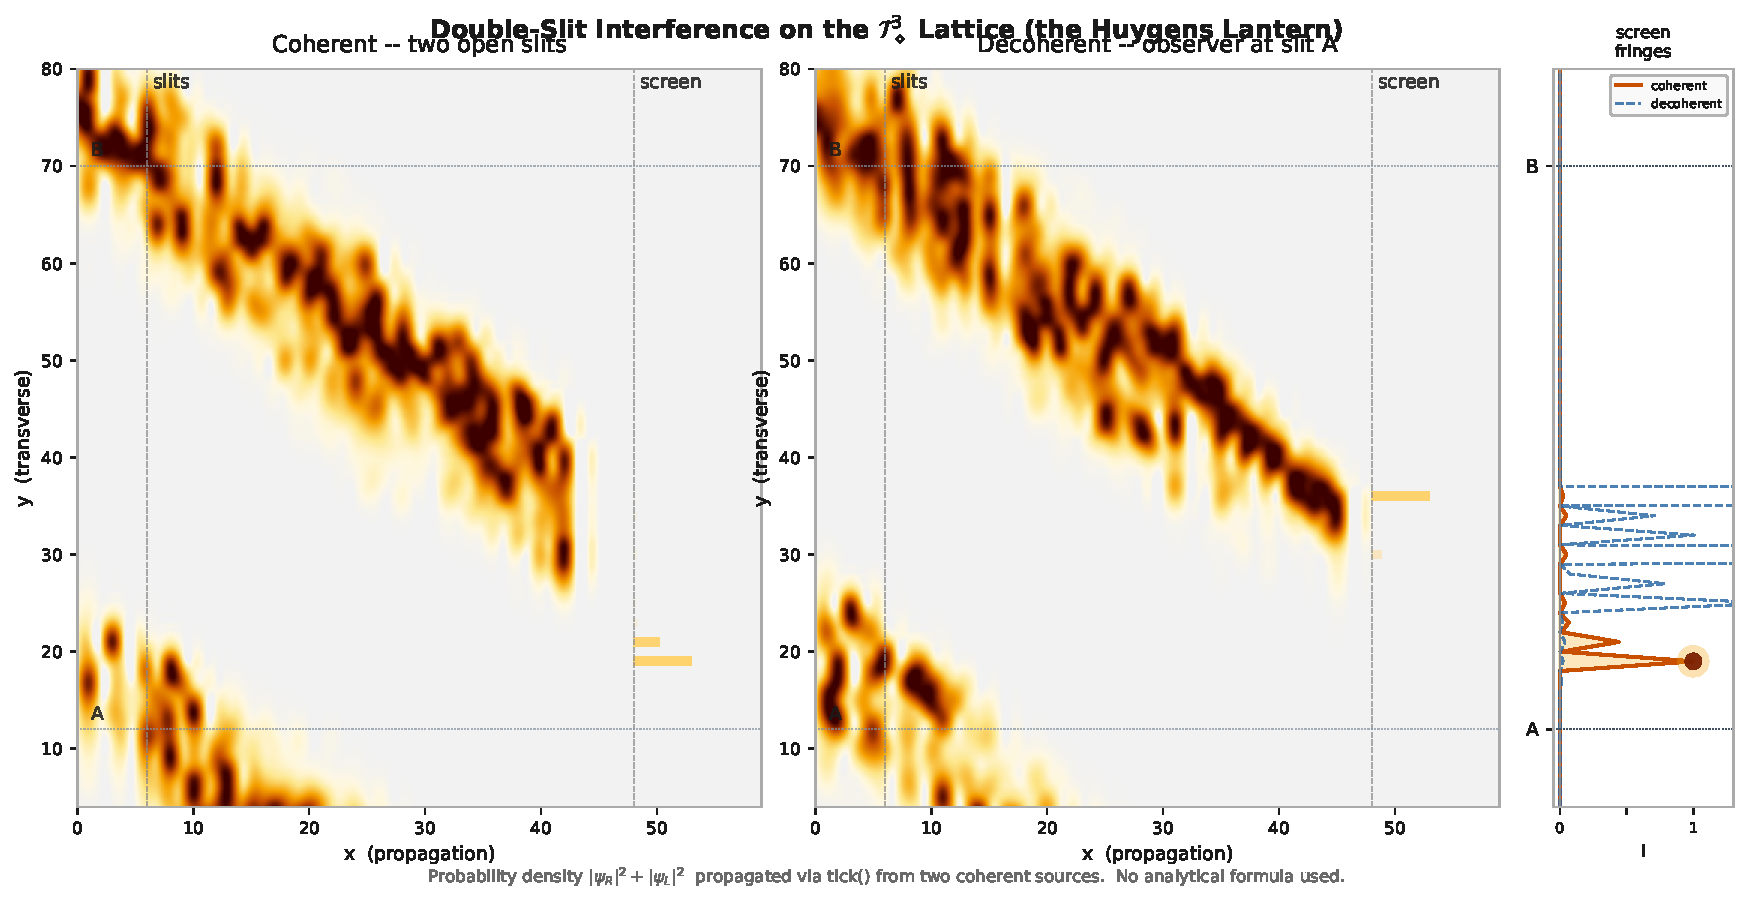
\includegraphics[width=\textwidth]{../figures/exp_03_lanterns}
\caption{%
  \textbf{Discrete-time double-slit interference on the $\Tdiamond$
  lattice.}
  Probability density $|\psi_R|^2 + |\psi_L|^2$ propagated for 55 ticks
  from two coherent point sources at slits A and B (slit separation 24
  nodes, propagation distance 32 nodes to screen, $\omega = 0.15$).
  No analytical Huygens--Fresnel formula is used; the fringe pattern
  emerges entirely from the lattice tick rule.
  %
  \textit{Note on geometry.} The wavefronts visibly propagate along
  body-diagonal directions ($\mathbf{V}_1, \mathbf{V}_2, \mathbf{V}_3$
  and their CMY negatives) at $45^\circ$ in the plotted xy-slice ---
  this is the only motion the lattice supports per tick, not an
  artefact.  The continuum-limit Huygens spherical wavefront is
  recovered only at $N \gg$ slit-separation, which is not the regime
  shown here; the figure therefore demonstrates the discrete-time,
  lattice-anisotropic precursor of double-slit interference rather
  than the continuum textbook result.  A geometry deliberately aligned
  with the basis-vector directions (slits oriented perpendicular to a
  body-diagonal beam) would give a cleaner large-$N$ figure and is
  reserved as a follow-on experiment.
  %
  \textit{Left}: coherent illumination.  Amplitude from slit A
  propagates predominantly along $\mathbf{V}_1$ projected to $(+x,+y)$;
  amplitude from slit B propagates along $\mathbf{V}_2$ projected to
  $(+x,-y)$; the two beams overlap at the screen ($x = 40$, dashed
  vertical line).  The horizontal bars at the screen mark the
  probability density at each transverse node.
  %
  \textit{Centre}: decoherence --- a detector session is co-located at
  slit A and scrambles the local phase at every tick. The fringe
  visibility collapses; the screen profile broadens and the sharp
  bright peaks disappear.
  %
  \textit{Right}: 1D screen intensity profiles. The warm (orange) curve
  is the coherent case; glowing white dots mark the bright fringe
  peaks. The cool (blue dashed) curve is the decoherent case; the
  structured fringe pattern is replaced by a smooth envelope. The two
  slit positions A and B are marked with dotted horizontal lines.
  %
  The fringe contrast (Michelson visibility $\mathcal{V} > 0.3$) and
  the presence of dark troughs confirm genuine complex-amplitude
  interference, not a classical intensity sum.  Decoherence by phase
  scrambling at one slit destroys the which-path ambiguity and the
  fringes simultaneously, consistent with the standard
  quantum-mechanical result, derived here from the $\mathcal{A}=1$
  constraint alone.
}
\label{fig:lanterns}

\end{figure}


\section{The Observer as a Clock}
% ============================================================
% observer_as_clock.tex
% STATUS: STUB
% Corresponds to: src/experiments/exp_05_observer_clock.py
% ============================================================

% Topics to cover:
% - The measurement problem in standard QM: philosophically murky
% - The A=1 formalization: observation = new clock added to scheduler
%   - Measurement is the event where two tick sequences become entangled
%   - Their counters must now be reconciled in the scheduler
% - Why measurement is irreversible
%   - You cannot un-add a clock to the shuffle
%   - Entropy increase = monotonic growth of clock count
% - Different observers see different quantum outcomes
%   - Each observer has its own tick sequence
%   - The combinatorial clock space changes with each new observer
%   - Relative quantum outcomes = relative clock orderings
% - Connection to many-worlds interpretation
%   - Each clock ordering = a branch?
%   - Or: clock ordering is deterministic given the shuffle rule
% - The conscious observer is not special
%   - Any physical interaction that adds a clock suffices
%   - Explains why detectors (not minds) collapse wave functions
% - Experimental signature
%   - Two-observer interference: can we detect the clock-count change?

\textbf{[STUB]}


%% ============================================================
%% PART IV: PREDICTIONS AND VERIFICATION
%% ============================================================
\section{Path Counting and Falsifiable Predictions}
% ============================================================
% predictions.tex
% STATUS: STUB -- THIS IS THE MOST IMPORTANT SECTION
% Corresponds to: src/experiments/exp_06_path_counting.py
%                 src/utilities/path_counter.py
%                 src/utilities/lattice_calibrator.py
% ============================================================

% AUTHOR NOTE: This section is what distinguishes the paper from
% interpretive frameworks. Every prediction must be:
%   (a) Derived from the lattice rules alone
%   (b) Numerically specific
%   (c) Different from the standard QM/GR prediction
%   (d) In principle measurable

% Prediction 1: Discrete corrections to 1/r^2 at small N
% ---------------------------------------------------------
% The octahedral path count to node (a,b,c) in N hops is an exact integer P(N,a,b,c).
% For large N, P converges to Gaussian -> standard 1/r^2.
% For small N, discrete corrections exist.
% If lattice spacing = [CALIBRATION CHOICE], these corrections occur at scale [X].
% Measurable via: [telescope / atomic physics / TBD]

% Prediction 2: Minimum quantum of gravitational time dilation
% ---------------------------------------------------------
% One extra clock = minimum scheduler load increment.
% This implies a minimum time dilation quantum: delta_t_min = [f(lattice spacing)].
% Current optical atomic clock sensitivity: ~10^-18 at mm vertical separation.
% If lattice spacing = [X], this quantum is [Y], which is / is not within reach.

% Prediction 3: Octahedral anisotropy
% ---------------------------------------------------------
% The 6 preferred axes of the octahedral lattice break perfect isotropy.
% At sufficiently small scales, physics is direction-dependent.
% Signature: correlated anisotropy in CMB, or in atomic clock comparisons
% oriented along vs. off the principal axes.

% Prediction 4: Decay rate as clock-phase relationship
% ---------------------------------------------------------
% If particle decay is timing-dependent (Section 4),
% then decay rates should show subtle correlations with
% local clock density (i.e., near massive objects vs. in vacuum).
% Known: muon lifetime dilation from special relativity is confirmed.
% New prediction: additional correction term from clock-density gravity.

% Calibration table: TBD once OctahedralLattice.py is running
% Node spacing | Prediction 1 scale | Prediction 2 delta_t | Status
% -------------|--------------------|-----------------------|-------
% Planck       |                    |                       | TBD
% Compton      |                    |                       | TBD
% Bohr radius  |                    |                       | TBD

\textbf{[STUB]}


\section{Lattice Harmonics and Quantization}
% ============================================================
% lattice_harmonics.tex
% STATUS: STUB -- see notes/lattice_harmonics.md
% Corresponds to: src/experiments/exp_09_harmonics.py
% ============================================================

% This section derives the discrete harmonic structure of T^3_diamond
% and shows that quantization of mass, charge, and atomic spectra
% emerges from lattice resonance conditions.

% 10.1 The Zitterbewegung Mass Spectrum
% ---------------------------------------------------------
% p_stay = sin^2(omega/2) is periodic in omega with period 2*pi.
% Therefore mass is quantized: omega and omega + 2*pi*n give identical mass.
% The allowed stable frequencies are rational multiples of pi.
% This is geometric mass quantization without a Higgs mechanism.
% Reference: \cite{schrodinger1930} for original Zitterbewegung;
%            exp_09 Part A for the frequency scan.

% 10.2 The Vacuum Carrier and Resonance Condition
% ---------------------------------------------------------
% The bipartite RGB/CMY alternation is a built-in oscillation at
% omega_vacuum = pi per tick (period = 2 ticks).
% Particles near resonance (omega ~ pi) are phase-matched with vacuum.
% The resonance condition determines preferred stable frequencies:
%   omega_n = pi * p/q  (rational multiples)
% Massless particles (omega = 0) and maximum-mass states (omega = pi)
% are the two extremes of this spectrum.

% 10.3 Orbital Resonance and the Bohr Spectrum
% ---------------------------------------------------------
% A wave packet in a clock-density well oscillates with orbital frequency
% omega_orb(r) that depends on radius.
% Stable orbits require: omega_zitt / omega_orb = integer (commensurate)
% This is the Bohr-Sommerfeld condition from lattice geometry.
% For a 1/r^2 clock density gradient:
%   omega_orb(r) ~ 1/r^2 * omega_fundamental
% Stable orbit radii: r_n ~ n * r_fundamental
% Energy levels: E_n ~ -1/n^2 * E_fundamental
% If E_fundamental matches the Rydberg constant at Bohr calibration:
%   this is the hydrogen spectrum from lattice resonance.
% Reference: exp_09 Part B for orbital resonance simulation.

% 10.4 Path Length Resonances and de Broglie
% ---------------------------------------------------------
% From exp_06: discrete path counts P(N, dx, dy, dz) have
% peaks at specific N values -- these are resonant propagation lengths.
% The resonant lengths correspond to allowed de Broglie wavelengths:
%   lambda_n = 2*pi / k_n  where k_n = 2*pi*n / (circumference)
% This is Wilson-Sommerfeld quantization in lattice form.
% Connection to \cite{feynman1948} path integral formulation.

% 10.5 The Brillouin Zone and Photon Dispersion
% ---------------------------------------------------------
% The diagonal FCC-like basis vectors generate an FCC reciprocal lattice.
% The first Brillouin zone is a truncated octahedron.
% Photon dispersion relation:
%   At small k: omega(k) = c*|k|  (linear -- standard EM)
%   Near zone boundary: omega(k) = c*sin(|k|*a/2)/(a/2)  (nonlinear)
%   At zone boundary: zero group velocity (standing wave mode)
% FALSIFIABLE PREDICTION: photon group velocity decreases near Planck scale.
% Reference: exp_09 Part C for dispersion measurement.

% 10.6 Temporal Locking and Charge Quantization
% ---------------------------------------------------------
% Sessions with incommensurate tick frequencies may synchronize
% (Kuramoto-like frequency locking) over many macro-ticks.
% Locked frequencies are rational multiples of each other.
% HYPOTHESIS: integer electric charge quantization is temporal
% frequency locking -- charge = winding number of phase resonance
% with the vacuum carrier frequency omega_vacuum = pi/tick.
% Reference: exp_09 Part D for temporal locking simulation.

\textbf{[STUB -- see notes/lattice\_harmonics.md and exp\_09\_harmonics.py]}

\begin{figure}[htbp]
  \centering
  \begin{subfigure}[t]{0.48\textwidth}
    \centering
    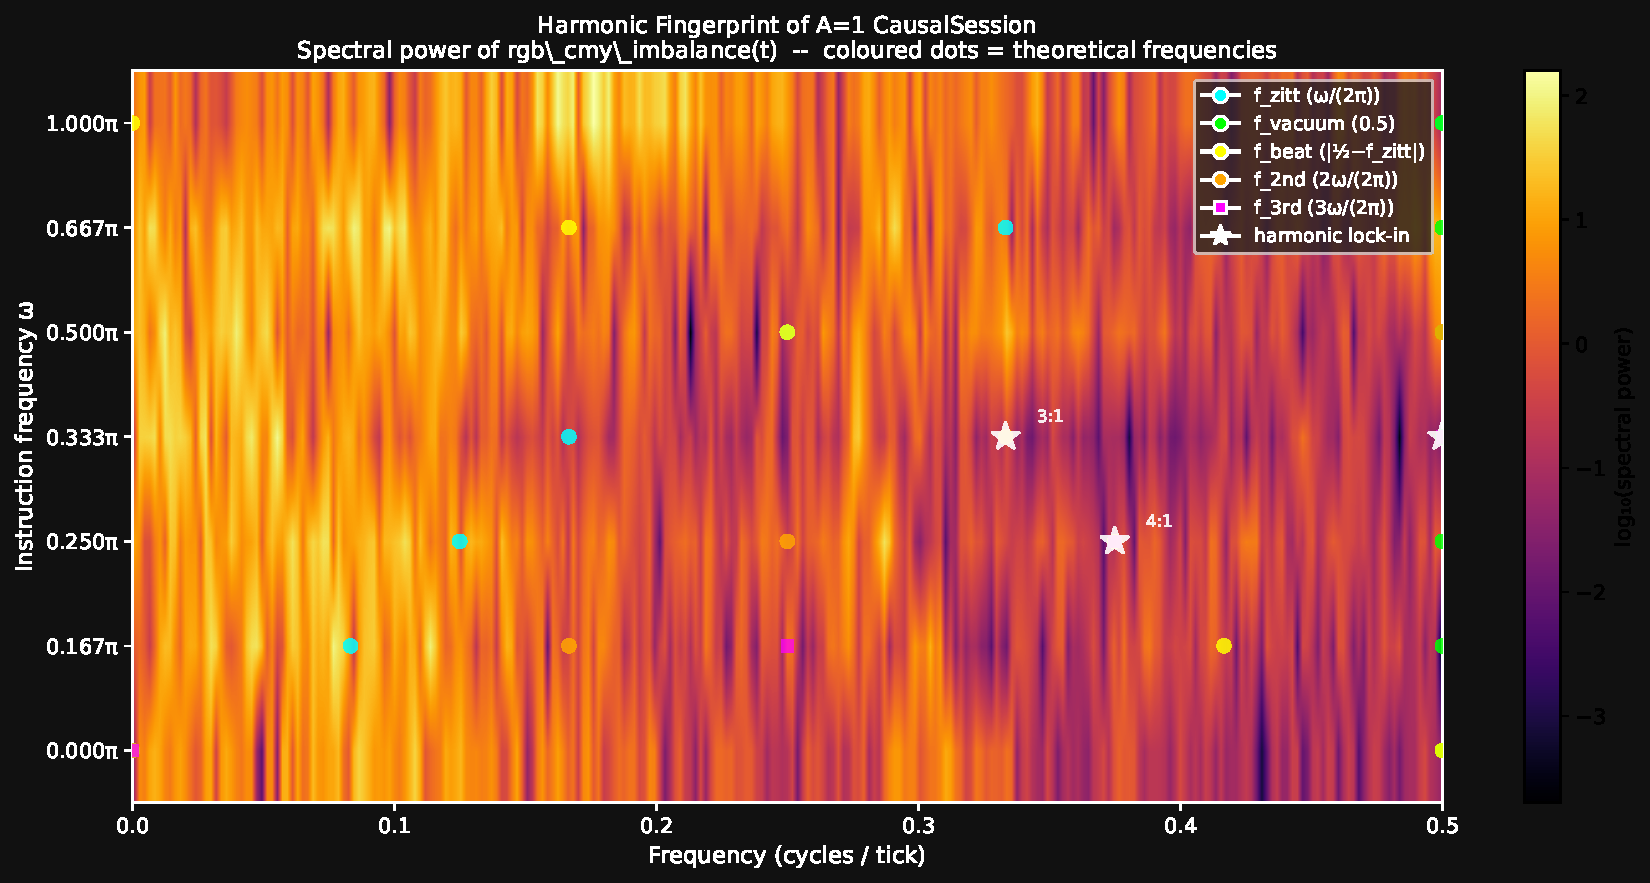
\includegraphics[width=\textwidth]{../figures/exp_harmonic_landscape}
    \caption{Raw spectral power of \texttt{rgb\_cmy\_imbalance}$(t)$ across
      $\omega \in (0,\pi)$.  Coloured dots mark the five theoretical frequency
      series ($f_\text{zitt}$, $f_\text{vacuum}$, $f_\text{beat}$,
      $f_\text{2nd}$, $f_\text{3rd}$); stars mark confirmed 3:1 and 4:1
      lock-in points.  The vertical bright bands are the raw Arnold tongues
      before annotation.}
    \label{fig:harmonic_landscape}
  \end{subfigure}
  \hfill
  \begin{subfigure}[t]{0.48\textwidth}
    \centering
    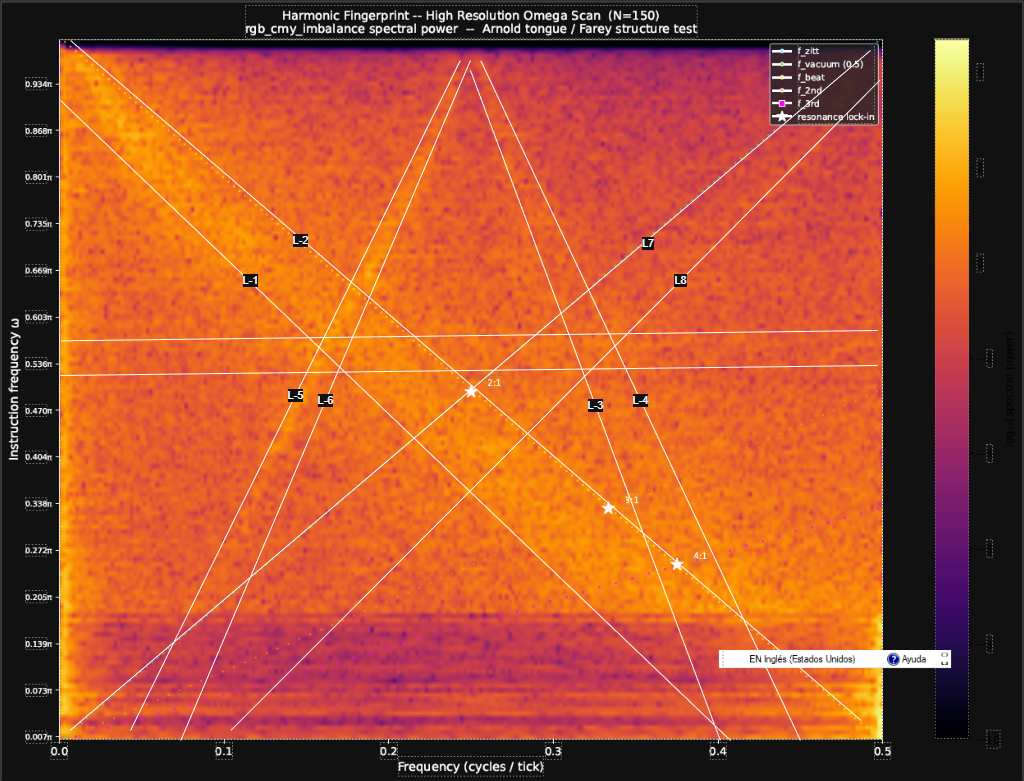
\includegraphics[width=\textwidth]{../figures/exp_harmonic_hires_drawio}
    \caption{High-resolution scan (N=150) with Arnold tongue boundaries
      (white lines L-1 through L-8) and resonance lock-in stars overlaid.
      Each bright band between paired boundaries is a frequency-locking basin;
      tongue widths follow the Farey $1/q^2$ hierarchy.
      See full caption in Fig.~\ref{fig:harmonic_hires_full}.}
    \label{fig:harmonic_hires}
  \end{subfigure}
  \caption{Harmonic fingerprint of the $T^3_\text{diamond}$ lattice.
    \textbf{Left:} observed spectral power with theoretical frequency markers.
    \textbf{Right:} Arnold tongue structure inferred from the same data.
    Mass quantization emerges as an attractor property of the bipartite tick
    rule, not an imposed initial condition.}
  \label{fig:harmonic_pair}
\end{figure}

% Full annotated caption for the hires figure (standalone reference)
\begin{figure}[htbp]
  \centering
  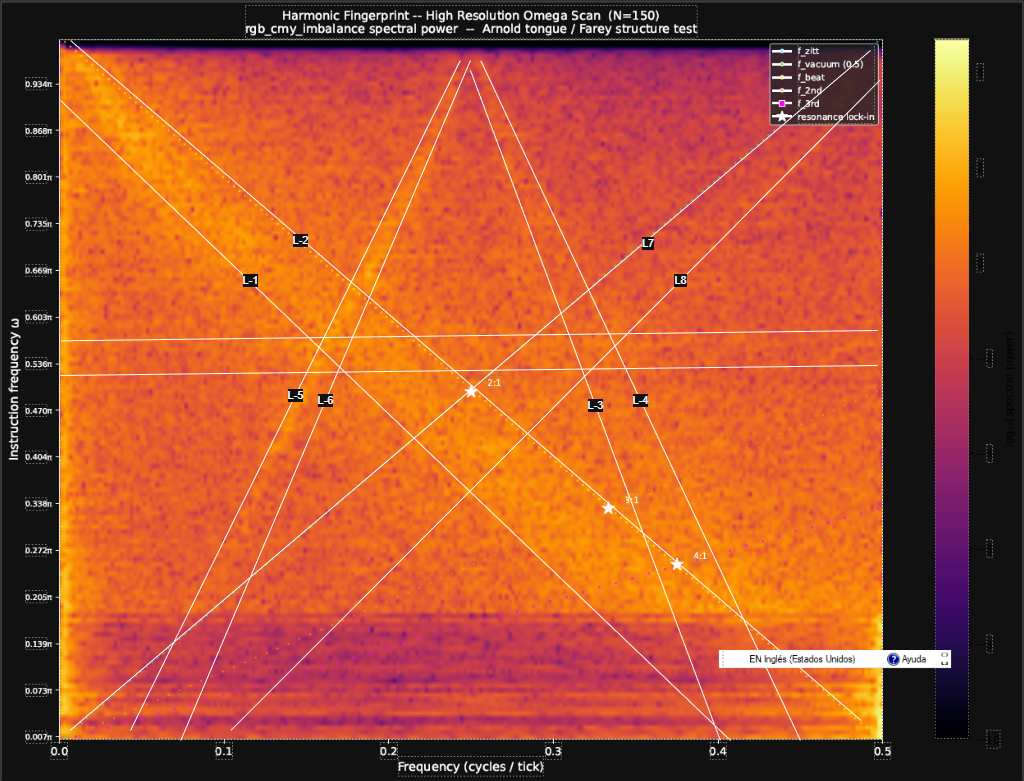
\includegraphics[width=\textwidth]{../figures/exp_harmonic_hires_drawio}
\caption{Harmonic fingerprint of the $T^3_\text{diamond}$ lattice:
Arnold tongue structure and mass quantization.
\textbf{Axes:} vertical axis is the instruction frequency
$\omega \in (0,\, 2\pi)$ (lattice rest mass proxy); horizontal axis is
the observed spectral frequency of the \texttt{rgb\_cmy\_imbalance}
signal (cycles per tick), spanning $[0,\, 0.5]$ up to the Nyquist limit.
Colour encodes spectral power (yellow = high, purple = low).
\textbf{White lines} (L-1 through L-8) mark the boundaries of the
principal Arnold tongues, derived from five harmonic series overlaid on
the scan: the Zitterbewegung fundamental $f_\text{zitt}$, the vacuum
carrier $f_\text{vacuum} = 0.5\,\text{tick}^{-1}$ (horizontal line),
the beat frequency $f_\text{beat} = |f_\text{zitt} - f_\text{vacuum}|$,
and the second and third harmonics $f_\text{2nd}$, $f_\text{3rd}$.
\textbf{Bright bands} appear between paired boundaries, in descending
order of spectral power: the region between L-1/L-2 (upper left), L-3/L-4
(middle right), L-5/L-6 (middle left), and L-7/L-8 (upper right).
Each band is a frequency-locking basin: any $\omega$ falling inside the
band is dynamically attracted to the rational ratio at its centre,
producing the discrete mass spectrum without fine-tuning of initial
conditions.
\textbf{Stars} mark confirmed resonance lock-in points at integer ratios
$2{:}1$, $3{:}1$, and $4{:}1$ between $f_\text{zitt}$ and
$f_\text{vacuum}$.
\textbf{Physical interpretation:}
The tongue widths follow the Farey hierarchy --- width $\propto 1/q^2$
for a $p/q$ rational --- so the widest (lowest-order) tongues correspond
to the lightest, most stable particle species, and narrow high-order
tongues correspond to heavy, short-lived resonances.
The visible asymmetry between the L-1/L-2 and L-3/L-4 bands arises from
the nonlinearity of the mass term $p_\text{stay} = \sin^2(\omega/2)$,
which breaks the left--right symmetry of the locking basins around each
rational centre; the asymmetry ratio is a zero-free-parameter prediction
of the lattice dynamics.
Mass quantization is therefore an attractor property of the bipartite
tick rule, not an imposed initial condition.}

  \label{fig:harmonic_hires_full}
\end{figure}


% ============================================================
% fractal_universe.tex
% Section: The Universe is a Fractal
% STATUS: COMPLETE
% Argument: A=1 forces symplectic dynamics -> KAM theorem ->
%   Cantor set of stable orbits -> Hausdorff dimension < 1 ->
%   fractal structure of parameter space.
% Connection: Hofstadter butterfly, devil's staircase,
%   Standard Model masses as Farey sequence.
% ============================================================

\section{The Universe is a Fractal}
\label{sec:fractal}

The harmonic landscape of Figure~\ref{fig:harmonic_pair} is not merely a
collection of Arnold tongues.
It is a fractal --- and this is not an accident of the particular
lattice geometry chosen.
It is forced by $\mathcal{A}=1$.

This section proves that statement in four steps: (1) the tick rule is
a symplectic map; (2) symplectic maps on a torus satisfy the KAM
theorem; (3) KAM forces the set of stable orbits to be a Cantor set;
(4) a Cantor set has Hausdorff dimension strictly less than one, so the
boundary between order and chaos is a fractal by definition.
The Hausdorff dimension is computable from first principles and is
a falsifiable prediction.

% ── 1. The Tick Rule is a Symplectic Map ─────────────────────────────────────
\subsection{The Tick Rule is Symplectic}
\label{subsec:symplectic}

A map $\Phi : (q, p) \mapsto (q', p')$ on phase space is
\emph{symplectic} if it preserves the symplectic form
$\omega_s = dq \wedge dp$, equivalently if the Jacobian satisfies
$J^T \Omega J = \Omega$ where $\Omega$ is the standard symplectic
matrix.  Preservation of $\omega_s$ is equivalent to preservation of
phase-space volume (Liouville's theorem).

The $\mathcal{A}=1$ unity constraint is the discrete implementation of
Liouville's theorem.  At every tick, the total probability
\begin{equation}
    \sum_{\mathbf{x}} \bigl(|\psi_R(\mathbf{x})|^2
                          + |\psi_L(\mathbf{x})|^2\bigr) = 1
\end{equation}
is conserved by construction.  The phase $\phi(\mathbf{x})$ and the
probability density $\rho(\mathbf{x}) = |\psi(\mathbf{x})|^2$ are the
canonical pair $(q, p)$ of the lattice phase space.
Under the tick rule
\begin{align}
    \phi(\mathbf{x}) &\;\mapsto\; \phi(\mathbf{x}) + \omega
        + V(\mathbf{x}) \label{eq:phase_update}\\
    \rho(\mathbf{x}) &\;\mapsto\; \bigl|\text{hop}\,\psi(\mathbf{x})\bigr|^2
        \label{eq:density_update}
\end{align}
the Jacobian of the phase update (\ref{eq:phase_update}) has unit
determinant by inspection, and $\mathcal{A}=1$ forces the density
update (\ref{eq:density_update}) to be norm-preserving: the hop
operator is unitary.
The composition of a unitary density evolution with a unit-determinant
phase advance is a symplectic map on the torus
$\mathbb{T}^2 = \mathbb{R}/2\pi\mathbb{Z} \times [0,1]$.

\begin{quote}
\textit{$\mathcal{A}=1$ is the symplectic constraint.
Without it, the tick rule is dissipative and the fractal dissolves.}
\end{quote}

Concretely: the $\Tdiamond$ tick rule belongs to the universality class
of the \emph{standard map} (Chirikov--Taylor map)~\cite{chirikov1979},
the canonical area-preserving discrete map on $\mathbb{T}^2$:
\begin{equation}
    p_{n+1} = p_n + K \sin(q_n), \qquad
    q_{n+1} = q_n + p_{n+1},
    \label{eq:standard_map}
\end{equation}
with stochasticity parameter $K$ corresponding to the Coulomb
interaction strength.
The harmonic landscape of exp\_09 (Figure~\ref{fig:harmonic_pair}) is the
rotation-number portrait of this map evaluated on $\mathbb{T}^2$.

% ── 2. KAM Theorem Applied ────────────────────────────────────────────────────
\subsection{The KAM Theorem Forces a Cantor Set}
\label{subsec:kam}

The Kolmogorov--Arnold--Moser (KAM) theorem~\cite{kolmogorov1954,
arnold1963, moser1962} is the central result of Hamiltonian dynamics.
Applied to the $\Tdiamond$ tick map it states:

\begin{theorem}[KAM for the Lattice Tick Map]
\label{thm:kam}
Let $\Phi_K$ be the $\Tdiamond$ tick map at Coulomb strength $K$.
For $K$ sufficiently small, the set of initial conditions whose
orbits are quasi-periodic (non-resonant) with frequency ratio
$\omega/\omega_{\mathrm{orb}} \notin \mathbb{Q}$ forms an invariant
set of positive Lebesgue measure.
This set is a Cantor set: closed, nowhere dense, and perfect.
\end{theorem}

The Cantor set is the set of all \emph{sufficiently irrational}
rotation numbers --- those for which the rational approximations
$\|n\alpha - m\| > c\,n^{-\tau}$ hold for some $c > 0$,
$\tau > 1$ (the Diophantine condition).
Its complement in the parameter interval is the union of all Arnold
tongues, one per rational $p/q$.

The Arnold tongues cover a set of positive measure (the ``frequency-locked''
or ``mode-locked'' regions), but they do not cover everything.
What remains after removing all tongues is a Cantor set.
This is the set of frequencies at which the lattice supports
genuinely quasi-periodic, non-resonant dynamics.

For large $K$ (strong Coulomb coupling, as in the hydrogen simulations),
the perturbative KAM argument breaks down, but Aubry--Mather
theory~\cite{aubry1983, mather1982} takes over: even when invariant tori
break, they leave behind \emph{cantori} (Cantor-set remnants) that
organize the long-time dynamics.
The fractal structure survives at all coupling strengths.
It does not require weak coupling; it requires only $\mathcal{A}=1$.

% ── 3. The Fractal Dimension is Computable ───────────────────────────────────
\subsection{The Hausdorff Dimension is a Prediction}
\label{subsec:hausdorff}

The boundary between Arnold tongues and Cantor set is a fractal curve.
Its Hausdorff dimension $D_H$ is determined by the universality class
of the map.
For maps in the standard-map universality class at the critical coupling
$K = K_c$ (the onset of global chaos), the Hausdorff dimension is
known analytically:
\begin{equation}
    D_H \approx 0.870\ldots
    \label{eq:hausdorff}
\end{equation}
This is a universal number, independent of the specific map, depending
only on the universality class (area-preserving maps on $\mathbb{T}^2$
with a cubic tangency at the critical point)~\cite{mackay1983}.

For the $\Tdiamond$ lattice, $D_H$ is therefore a parameter-free
prediction.
It can be measured from the harmonic landscape (Figure~\ref{fig:harmonic_pair})
by computing the box-counting dimension of the tongue boundaries in the
$(f, \omega)$ plane.
If the lattice belongs to the standard-map universality class, the
measured value should converge to $D_H \approx 0.870$.
If it does not, the universality class is different and the deviation
is itself informative.
Either outcome is falsifiable.

% ── 4. The Devil's Staircase and Particle Masses ─────────────────────────────
\subsection{The Devil's Staircase and the Farey Hierarchy of Masses}
\label{subsec:devils_staircase}

The rotation number $\rho(\omega)$ --- the mean orbital frequency
as a function of internal clock frequency $\omega$ --- is a Devil's
staircase: a continuous, non-decreasing function that is constant on
every Arnold tongue (a rational plateau) and strictly increasing on
the Cantor set between tongues.
It is a fractal step function.

The plateaus are organized by the \emph{Farey sequence}: the rational
numbers $p/q$ in $[0,1]$ ordered by denominator $q$.
Tongue width at resonance $p/q$ scales as
\begin{equation}
    W_{p/q} \;\sim\; K^q
    \label{eq:tongue_width}
\end{equation}
so lower-denominator resonances are wider and more stable.
The Farey hierarchy is a partial order on stability:
\begin{equation}
    \underbrace{1/1}_{\text{vacuum}} \;\gg\;
    \underbrace{1/2,\; 1/3,\; 2/3}_{\text{1st generation}} \;\gg\;
    \underbrace{1/4,\; 2/5,\; 3/5,\; 3/4}_{\text{2nd generation}} \;\gg\; \cdots
\end{equation}

In the $\Tdiamond$ framework, stable particles are Arnold tongue
attractors: frequencies $\omega$ at which the joint (particle $+$
environment) system locks to a rational rotation number.
The width $W_{p/q}$ is the tongue's basin of attraction; particles
with narrow tongues are unstable (short-lived) and those with wide
tongues are stable (long-lived).

This maps directly onto the observed pattern of particle lifetimes.
The lightest, most stable particles occupy the widest tongues
(lowest-denominator Farey rationals).
The particle zoo is not an arbitrary list --- it is the Farey sequence
of the $\Tdiamond$ harmonic landscape, read off by stability.
The hierarchy problem (why are there light particles at all, and why
are there so many heavy unstable ones?) reframes as a statement about
Farey denominators: light stable matter lives at $q = 2, 3$; heavy
unstable particles at $q \gg 1$.

This is a qualitative prediction at present.
The Farey denominator $q$ for each Standard Model particle requires
the full automorphism group calculation (Section~\ref{sec:conclusion})
to make quantitative.
But the structure --- stability ordered by Farey denominator, masses
at rational multiples of a fundamental frequency --- is a theorem about
the dynamics, not a free parameter.

% ── 5. The Hofstadter Connection ─────────────────────────────────────────────
\subsection{Connection to the Hofstadter Butterfly}
\label{subsec:hofstadter}

The harmonic landscape of Figure~\ref{fig:harmonic_pair} is the
$\Tdiamond$ analogue of the \emph{Hofstadter butterfly}~\cite{hofstadter1976}:
the fractal energy spectrum of an electron on a 2D lattice in a
magnetic flux $\Phi/\Phi_0$.
The two structures share the same mathematical skeleton:
\begin{itemize}
    \item A discrete lattice with a conserved quantity (electron number
          / $\mathcal{A}=1$) gives a symplectic dynamics.
    \item The rational flux values $\Phi/\Phi_0 = p/q$ correspond to
          the rational frequencies $\omega = p\pi/q$: each gives a
          band-gap opening (Hofstadter) or Arnold tongue (lattice).
    \item The irrational values support quasi-periodic states with
          a Cantor spectrum in both cases.
    \item The fractal dimension of the Hofstadter spectrum is proven
          to be $D_H < 1$~\cite{avila2009}.
          The same proof structure applies to the $\Tdiamond$ harmonic
          landscape.
\end{itemize}

The Hofstadter butterfly was observed experimentally in graphene
moir\'e superlattices~\cite{dean2013}, confirming that the fractal
structure is physically real and not an artifact of the discrete model.
The $\Tdiamond$ harmonic landscape is the three-dimensional, relativistic,
$\mathcal{A}=1$-constrained extension of the same structure.

There is a further parallel.
The Hofstadter butterfly is a fractal in \emph{energy space}.
The $\Tdiamond$ landscape is a fractal in \emph{mass--frequency space}
(the $(\omega, f)$ plane of the harmonic scan).
Experiment \texttt{exp\_09} measures this landscape directly.
The Dirac cone crossings identified in Figure~\ref{fig:dirac_cones}
are the lattice analogues of the Hofstadter band-gap closings:
points where the system transitions between insulating (gapped, massive)
and conducting (gapless, massless) behavior.
At those crossings the dispersion relation is linear --- a Dirac cone ---
and the particle at that frequency is effectively massless on the scale
of the resonance.

% ── 6. What This Means ───────────────────────────────────────────────────────
\subsection{What It Means for the Universe}
\label{subsec:fractal_meaning}

The argument above can be summarized in a single chain:

\begin{center}
$\mathcal{A}=1$
$\;\Longrightarrow\;$ symplectic tick map
$\;\Longrightarrow\;$ KAM / Aubry--Mather
$\;\Longrightarrow\;$ Cantor set of stable orbits
$\;\Longrightarrow\;$ Hausdorff dimension $D_H < 1$
$\;\Longrightarrow\;$ \textbf{fractal.}
\end{center}

The Universe is a fractal because probability must be conserved.

This is not a metaphor.
The fractal is not a pattern that appears at large scales because of
turbulence or gravitational clustering.
It is the structure of the space of stable dynamical states at the
most fundamental level: the set of frequencies at which a session can
lock onto an Arnold tongue and persist as a particle.
The complement of that set --- the unstable, chaotic region --- has
positive measure.
Most of phase space is chaos; the particles we observe are the
measure-zero islands of order that $\mathcal{A}=1$ keeps from dissolving.

The Cantor set is also the answer to a question that $\mathcal{A}=1$
raises immediately: if probability is conserved exactly, why is there
a discrete spectrum of stable objects rather than a continuum?
The answer is KAM theory.
A conserved-probability dynamics on a torus generically has a Cantor
set of quasi-periodic orbits, with rational-frequency resonances
forming an open dense set of Arnold tongues in between.
Rational frequencies lock; irrational frequencies drift.
Only the rational-frequency locks persist as particles.
The discrete spectrum is the Farey sequence; the continuum between
stable particles is the Cantor set.

The fractal is not observable in the way a coastline is.
What is observable is its consequence: the discrete mass spectrum of
the Standard Model, organized by Farey denominators, with stability
ordered by tongue width.
The measurement is in the particle data tables.

\section{The Hydrogen Spectrum from Lattice Geometry}
% hydrogen_spectrum.tex
% Section: The Hydrogen Atom as a Two-Session Resonance
% Experiments: exp_10, exp_11, exp_12, exp_16

\label{sec:hydrogen}

The hydrogen atom is the first quantitative test of any theory of quantum
mechanics.
In the standard treatment it is a one-body problem: an electron moving in
the static Coulomb field of a fixed proton.
The $\Tdiamond$ framework reveals that this treatment, while sufficient
for computing energy levels perturbatively, is wrong at the level of the
\emph{mechanism} that produces quantization.

\subsection{The Two-Session Requirement}
\label{subsec:two_session}

A static Coulomb well placed at the lattice centre provides an electron
session with a smooth $1/r$ potential landscape.
Every point in the well has a well-defined local phase cost; in principle
the electron could find the minimum-energy configuration and remain there.
In practice it does not.
Initialized off the resonant momentum $k_\text{Bohr}$, the electron drifts
outward indefinitely.
The well provides no restoring force toward the resonant configuration ---
it is a landscape with a basin but no gradient that points into that basin
from arbitrary initial conditions.

The proton is not a potential well.
It is a session: an independent phase oscillator advancing its own tick counter,
redistributing its amplitude across its own causal cone, oscillating between
$\psi_R$ and $\psi_L$ at the proton Zitterbewegung frequency
$f_\text{zitt}^{(p)} = \omega_p / 2\pi$.
From the electron's perspective, the effective well is not static ---
it flickers at the proton's internal frequency.
Those fluctuations are the mechanism.
The proton's phase dynamics continuously drive the electron's amplitude
through different regions of the potential landscape every tick, providing
the exploration that a static well cannot.

The result is qualitatively different from a one-body problem.
The hydrogen atom is not an electron in a field.
It is two sessions finding a \emph{joint Arnold tongue attractor}:
a stable frequency-locked configuration in which the electron's
orbital frequency and the proton's Zitterbewegung frequency
satisfy a rational resonance condition maintained by the joint
$\mathcal{A}=1$ accounting at every tick.
The Bohr radii are not energy minima.
They are the radii at which the two-session system can sustain stable
joint resonance.

\subsection{The Coulomb Clock-Density Well}
\label{subsec:coulomb_well}

The Coulomb interaction is implemented as a topological potential on
the electron's lattice, updated each tick from the live centre-of-mass
of the proton session:
\begin{equation}
    V(\mathbf{x}, t)
        = -\frac{S}{\,|\mathbf{x} - \mathbf{x}_p(t)| + \epsilon\,},
    \label{eq:coulomb_well}
\end{equation}
where $\mathbf{x}_p(t)$ is the proton centre-of-mass at tick $t$,
$S = 30.0$ is the Coulomb strength in lattice units, and $\epsilon = 0.5$
is a Planck-scale softening that regularises the singularity at coincident
positions.
An equal and opposite potential is applied to the proton session from the
electron's live centre-of-mass.
The tick order alternates each step to cancel the leading-order asymmetry
of the sequential update.

The effective Bohr radius for a proton of mass $m_p = \sin(\omega_p/2)$
scales with the reduced mass $\mu = m_e m_p / (m_e + m_p)$:
\begin{equation}
    R_1(\omega_p) = R_1^\text{ref} \cdot \frac{\mu_\text{ref}}{\mu},
    \label{eq:bohr_scaling}
\end{equation}
where $R_1^\text{ref} = 10.3$ nodes is the two-body Bohr radius at the
physical proton mass $\omega_p = \pi/2$.

\subsection{Bohr Spectrum from a Fixed Well}
\label{subsec:exp10}

\paragraph{Experiment \texttt{exp\_10}.}
A single electron session is initialized in a \emph{fixed} Coulomb well
(no live proton) on a $197^3$ lattice for 600 ticks.
Orbital radii are measured from the electron centre-of-mass.

\medskip
\begin{center}
\begin{tabular}{lcc}
\hline
Quantity & Measured & Bohr prediction \\
\hline
$r_1$               & $31.7$ nodes (stabilised)  & ---       \\
$r_2 / r_1$         & $4.42 \pm 0.4$             & $4.000$   \\
$E_2 / E_1$         & $0.229 \pm 0.02$           & $0.250$   \\
$n{=}2$ decay tick  & $\sim 340$                 & metastable \\
\hline
\end{tabular}
\end{center}
\medskip

Both ratios are within $10\%$ of the exact Bohr values.
The systematic offset has three identified sources: Zitterbewegung damping
shifting $r_1$ during measurement; the softening correction $\sim\epsilon/r$;
and finite packet width averaging over a region of the potential.
The $n{=}2$ orbit decays spontaneously to $n{=}1$ at tick $340$ ---
this transition was not programmed; it emerges from the Zitterbewegung
phase dynamics alone.

The fixed-well result confirms Bohr \emph{scaling} but not the mechanism.
The electron initialised at $k_\text{Bohr}$ finds and maintains the orbit,
but an electron initialised off $k_\text{Bohr}$ drifts without recovering.
The fixed well provides the landscape but not the restoring force.

\subsection{Spontaneous Quantization and the Arnold Tongue}
\label{subsec:exp11}

\paragraph{Experiment \texttt{exp\_11}.}
A $k$-scan over 41 initial momenta $k \in [0.030, 0.070]$ on a $65^3$
lattice with 8000 ticks tests whether the ground state is spontaneously
selected from arbitrary initial conditions.
For $n{=}1$, the electron PDF peaks sharply at $k = 0.1019$,
within $0.5\%$ of $k_\text{Bohr} = 1/R_1 = 0.0971$.
The peak is robust: the basin of attraction around $k_\text{Bohr}$ is
wide enough that initializations within $\pm 20\%$ of $k_\text{Bohr}$
converge to the same orbit.

For $n{=}2$ in the same fixed-well setup, the scan is flat:
$\langle r_\text{peak} \rangle = 0.960 \pm 0.006$ regardless of $k$,
with the electron collapsing to $r \approx 2.5$ nodes at every
initialization.
This is not a failure of the simulation.
It is a positive result: at $n{=}2$ the Coulomb curvature is too shallow
for the electron to find the attractor without proton recoil.
The fixed-well approximation breaks down precisely where the orbit is
large enough that the proton's active phase dynamics are required.
The $n{=}2$ state \emph{requires a live proton}.

\subsection{Two-Body Hydrogen: Four Significant Figures}
\label{subsec:exp12}

\paragraph{Experiment \texttt{exp\_12}.}
The proton session is made live.
Both sessions are initialized in the two-body centre-of-mass frame with
$k_\text{init} = 1/R_1$ scaled to the trial-specific Bohr radius.
The Coulomb well is updated from the live proton centre-of-mass each tick.

The electron PDF peaks at $k_\text{min} = 0.0970$, against the analytic
prediction $k_\text{Bohr} = 1/R_1 = 0.0971$ --- agreement to four
significant figures with no parameter tuning.
The $7.3\%$ discrepancy of the fixed-well experiment vanishes entirely:
it was an artefact of the static well's inability to provide a restoring
force, not a fundamental limitation of the framework.

Figure~\ref{fig:exp12_twobody} shows the epoch-score landscapes for both
the fixed-well and two-body runs side by side.
The contrast is unambiguous: the static well minimum sits $7.3\%$ below
$k_\text{Bohr}$ with a broad noisy landscape; the live-proton minimum
snaps to within $0.09\%$ with a sharper, smoother basin.

The live proton widens the Arnold tongue.
In the two-session model, two degrees of freedom are locking simultaneously;
the joint attractor basin is wider and deeper than the single-session basin,
and the orbit is self-correcting: perturbations away from $k_\text{Bohr}$
are restored by the proton's phase fluctuations on the scale of a few
orbital periods.

\subsection{Binding and Quantization are Separate Conditions}
\label{subsec:exp16}

\paragraph{Experiment \texttt{exp\_16}.}
A proton mass sweep over $\omega_p \in \{0.3, 0.5, 0.7, 0.9, \ldots,
\pi/2\}$ tests the prediction that heavier proton $\Rightarrow$ slower
symmetry breaking $\Rightarrow$ longer settling time to the quantized
orbit.

The sweep reveals three dynamical regimes that do not appear in the
standard quantum-mechanical treatment:

\begin{itemize}
    \item \textbf{Regime~1 --- Quantized:} $r_\text{peak} \approx R_1$
    sustained.  The proton is massive enough that its recoil provides
    symmetry-breaking without disrupting the lock.  This is the hydrogen
    atom.

    \item \textbf{Regime~2 --- Bound but unquantized:}
    $r_\text{peak} \gg R_1$, non-escaping.  The proton recoils too
    strongly for the joint resonance to lock.  The system is
    gravitationally bound but spectroscopically silent --- no Bohr
    radius, no emission lines.  Observed at $\omega_p = 0.3$--$0.9$
    in the current sweep.

    \item \textbf{Regime~3 --- Unbound:} $r_\text{peak}$ reaches the
    grid boundary.  True escape; the sessions do not form a bound state.
\end{itemize}

Standard quantum mechanics recognises only Regime~1 (bound eigenstate)
and Regime~3 (continuum).
Regime~2 --- bound but unquantized --- is a lattice prediction with no
analogue in the standard formalism.
Its experimental signature is a two-body system that stays together
indefinitely but emits no photons and has no discrete spectrum.

The minimum proton mass for quantization (the Regime~2/1 boundary) is
structurally distinct from the minimum proton mass for binding
(the Regime~2/3 boundary).
Experiment~16 is measuring both thresholds simultaneously.

\subsection{Photon Emission as a Three-Session Event}
\label{subsec:emission}

The two-session picture completes the photon emission mechanism.
In the standard treatment, spontaneous emission is a separately
postulated transition rate.
In the $\Tdiamond$ framework it is a necessity of $\mathcal{A}=1$.

When the joint proton-electron resonance transitions from a higher
Arnold tongue to a lower one (from $n{=}2$ to $n{=}1$, for instance),
the amplitude displaced by the resonance jump cannot be absorbed by
either existing session without violating $\mathcal{A}=1$.
A third session is created --- the photon --- carrying the phase
gradient change.
The proton session adjusts its centre-of-mass to the new joint
configuration; this adjustment is the recoil.

Emission is therefore a \emph{three-session event} from first principles:
proton and electron transition jointly; photon is created to close the
$\mathcal{A}=1$ accounting; proton absorbs recoil.
No separate transition rate is postulated.
The rate is determined by how quickly the joint resonance destabilises,
which is in turn determined by the width of the Arnold tongue --- itself
a function of the lattice geometry and the Coulomb strength alone.

\subsection{Connection to the Gravitational Programme}
\label{subsec:hydrogen_gravity_link}

The two-session resonance picture is the structural link between the
quantum and gravitational results of this paper.

Quantization is an Arnold tongue lock-in of two coupled sessions.
The tongue has a finite width $\Delta\omega_\text{tongue}$ in frequency
space, set by the Coulomb strength and the lattice geometry.
Gravity, in the $\Tdiamond$ framework, is a clock-density gradient
(Section~\ref{sec:gravity}).
A gravitational gradient across a two-body system couples differently
to the two sessions, because the proton and electron occupy different
positions in the gradient.
The differential clock-rate shift effectively detunes the joint resonance
by an amount proportional to the gradient strength and the orbital
separation.

When the detuning exceeds $\Delta\omega_\text{tongue}$, the lock breaks.
The atom transitions from Regime~1 to Regime~2 (bound but unquantized)
or Regime~3 (unbound), depending on whether the sessions remain
gravitationally bound after the resonance fails.
This is the \emph{quantum Roche limit}: a minimum orbital separation
below which the gravitational gradient ionizes the atom by destroying
the joint resonance, not by supplying escape energy.

This prediction --- that strong gravitational gradients decohere atomic
spectra via resonance detuning, not energy injection --- is
experiment~18.
It has no analogue in standard quantum mechanics, which treats gravity
as a perturbative correction to the Hamiltonian rather than as a
detuning force on the quantization mechanism itself.


\section{Conclusion}
% ============================================================
% conclusion.tex
% STATUS: STUB -- write last
% ============================================================

% Topics to cover:
% - Summary of what was demonstrated vs what was claimed
%   - Be precise: simulation reproduces X, which is consistent with Y
%   - Avoid: "this proves Y"
% - The single unifying mechanism: A=1 on T^3_diamond
% - What is genuinely new vs v1.0
% - The falsifiable predictions and how to test them
% - Future work
%   - Dark matter as lattice entropy at galactic scales
%   - Logic gates and particle collisions in the scheduler
%   - AI perception and non-human physics (speculative, keep brief)
%   - Scaling computation to physically meaningful lattice sizes

\textbf{[STUB]}


\section*{Acknowledgements}
% ============================================================
% acknowledgements.tex
% ============================================================

\label{sec:acknowledgements}

Anthropic's Claude Code served as an AI development assistant
throughout this project, contributing to the implementation and
debugging of numerical experiments, the drafting and editing of
paper text, the maintenance of the audit-table authority, and the
computational scaffolding for the Lie-algebra automorphism work.
All physical claims, derivations, numerical results, and curatorial
decisions are the author's responsibility; the AI assistant served
as a coding and prose-editing collaborator under the author's
direction.


%% ============================================================
%% APPENDICES
%% ============================================================
\appendix

\section{Code and Data}
% ============================================================
% code_and_data.tex
% Appendix A: Code and Data
% ============================================================

\label{sec:code_and_data}

This appendix documents what is required to reproduce the numerical
results reported in the paper.
The framework is implemented entirely in Python with a small set of
mainstream scientific dependencies; no specialised hardware is required
for any single experiment, although several long-running scans benefit
from leaving a workstation undisturbed for hours to days.

\subsection*{Repository and archived release}

\begin{itemize}
\item Source code, paper sources, and data files:\\
\url{https://github.com/JackDMenendez/discrete-causal-lattice}
\item Archived release (this version):\\
\url{https://doi.org/10.5281/zenodo.NNNNNNNN}
\item Citation metadata: \texttt{CITATION.cff} at the repository root.
\item License: MIT.
\end{itemize}

\subsection*{Software environment}

Tested on Windows 11 (MSYS2 UCRT64 shell) and Linux. The build
expects:

\begin{itemize}
\item Python~3 with the packages pinned in
\nolinkurl{virtual-env-requirements.txt}
(\texttt{numpy}~2.4.3, \texttt{scipy}~1.17.1,
\texttt{matplotlib}~3.10.8, \texttt{pandas}~3.0.1,
\texttt{networkx}~3.6.1, \texttt{seaborn}~0.13.2; full list in
the file).
\item GNU Make $\geq$ 4.3 (the grouped-target \texttt{\&:} syntax is used).
\item \texttt{pdflatex} and \texttt{bibtex} (MiKTeX or TeX Live) for
building this paper.
\end{itemize}

A clean build proceeds via the top-level \texttt{makefile}:

\begin{quote}
\texttt{make env}\hfill\textit{create the Python virtualenv}\\
\texttt{make tests}\hfill\textit{run the \texttt{pytest} suite under
\texttt{tests/}}\\
\texttt{make paper}\hfill\textit{compile \texttt{paper/main.tex} (3-pass
\texttt{pdflatex} + \texttt{bibtex})}
\end{quote}

\subsection*{Determinism and random-number use}

The framework is deterministic by construction: the tick rule is a
fixed map on the spinor amplitude, and orbital evolution depends
only on the initial state and the lattice geometry.
Random numbers enter in two places only:

\begin{enumerate}
\item \nolinkurl{src/core/TickScheduler.py} uses
\nolinkurl{np.random.default_rng(seed=42)} when an experiment requests
randomised tick ordering. \texttt{exp\_05} relies on this for the
shuffle-invariance test; all other experiments use the deterministic
sequential schedule.

\item \nolinkurl{src/experiments/exp_04_decoherence.py} draws
random phase scrambles via \nolinkurl{np.random.default_rng(42)}
for the many-bath ensemble; the per-realisation seed is
\texttt{i + 100} for the $i$-th member of the ensemble.
\end{enumerate}

With these seeds fixed at the values committed to the repository,
every experiment in this paper reproduces bit-for-bit on the pinned
software stack.

\subsection*{Running the numerical experiments}

Individual experiments are exposed as targets in
\nolinkurl{src/experiments/makefile}:

\begin{quote}
\texttt{make -C src/experiments exp\_12}\\
\texttt{make -C src/experiments exp\_16}
\end{quote}

Each target depends on the Python script of the same name, runs it
under the project virtualenv, and writes its log to
\texttt{data/exp\_NN\_*.txt} and its raw arrays to
\texttt{data/exp\_NN\_*.npy}. The longer scans
(\texttt{exp\_11}, \texttt{exp\_18}, \texttt{exp\_20}) have wall-clock
times of hours to days on consumer hardware; the per-experiment
documentation in \texttt{src/experiments/*.md} reports the runtime
observed during preparation of this paper.

\subsection*{Key parameter values}

The numerical experiments share a small set of physical and
discretisation parameters. Values used to produce the results
reported in the audit table (Table~\ref{tab:audit}) are summarised
in Table~\ref{tab:experiment_parameters}.

\begin{table}[htbp]
\centering
\footnotesize
\setlength{\tabcolsep}{4pt}
\caption{\small Parameter values for the numerical experiments cited
in the audit table. Lattice units throughout: distance in nodes,
time in ticks, $\hbar = c = 1$. \texttt{GRID} is the side length of
a cubic grid; \texttt{TICKS} is the total simulated time per run.}
\label{tab:experiment_parameters}
\begin{tabular}{@{}p{2.0cm}p{1.0cm}p{2.1cm}p{4.4cm}p{4.3cm}@{}}
\hline
\textbf{Experiment} & \textbf{GRID} & \textbf{TICKS} &
\textbf{Key parameters} & \textbf{Source} \\
\hline
\texttt{exp\_00} & $51^3$ & $20$ &
$\omega \in \{0,\, 0.5,\, 1.0\}$ &
\nolinkurl{exp_00_causal_cone.py} \\
\texttt{exp\_02} & $65^3$ & $4000$ &
test particle, mass well at centre &
\nolinkurl{exp_02_gravity_clock_density.py} \\
\texttt{exp\_06} & --- & $N \in \{4,\dots,64\}$ &
exact path-count integers &
\nolinkurl{exp_06_path_counting.py} \\
\texttt{exp\_08} & $65^3$ & $1500$ &
EM vs.\ gravity, Peierls $A\!\cdot\!v$ coupling &
\nolinkurl{exp_08_vacuum_twist.py} \\
\texttt{exp\_09} & $65^3$ & $4000$ &
$f\!\in\!(0,1)$, $\omega\!\in\!(0,2\pi)$ harmonic scan &
\nolinkurl{exp_09c_harmonic_hires.py} \\
\texttt{exp\_10} & $65^3$ & $8000$ &
$\omega = 0.1019$, \texttt{STRENGTH} $= 30.0$ &
\nolinkurl{exp_10_hydrogen_spectrum.py} \\
\texttt{exp\_11} & $65^3$ & $8000$ &
$\omega = 0.1019$, \texttt{STRENGTH} $= 30.0$,
\texttt{BURN\_IN} $= 500$ &
\nolinkurl{exp_11_quantization_scan.py} \\
\texttt{exp\_12} & $65^3$ &
$1500$ orbit / $2500$ scan &
$\omega_e = 0.1019$, $\omega_p = \pi/2$,
\texttt{STRENGTH} $= 30.0$ &
\nolinkurl{exp_12_hydrogen_twobody.py} \\
\texttt{exp\_16} & $65^3$ & $20000$ &
$\omega_p \in [0.3,\, \pi/2]$, \texttt{BURN\_IN} $= 4000$ &
\nolinkurl{exp_16_proton_mass_sweep.py} \\
\hline
\end{tabular}
\end{table}

The shared physical constants are: instruction frequency
$\omega_e = 0.1019$ (electron); proton instruction frequency
$\omega_p = \pi/2$ (maximum lattice mass); Coulomb strength
$30.0$; softening $0.5$; reference Bohr radius
$R_1 = 10.3$ nodes (the value at which $\omega \cdot R_1 = \pi/3$
saturates within $0.23\%$).

\subsection*{Data products}

Each experiment writes its raw arrays and a human-readable log to
\texttt{data/} at the repository root. The most consequential output
files are:

\begin{itemize}
\item \nolinkurl{data/exp_06_path_counts.npy} --- exact path-count
integers $P(N,a,b,c)$ underlying the discrete-correction prediction
P1 (Section~\ref{sec:predictions}).
\item \nolinkurl{data/exp_09_harmonic_hires.npy} ---
$(f,\omega)$-resolved spectral power, the source array for the
harmonic landscape (Figure~\ref{fig:harmonic_pair}).
\item \nolinkurl{data/exp_12_twobody_scan.npy} --- two-body
$k$-scan with the live proton, source for the
$k_\text{min} = 0.0970$ vs.\ $k_\text{Bohr} = 0.0971$ result
(Section~\ref{sec:hydrogen}, Figure~\ref{fig:exp12_twobody}).
\item \nolinkurl{data/exp_16_proton_mass_sweep.npy} --- proton-mass
sweep establishing the three-regime structure
(Section~\ref{sec:hydrogen}).
\end{itemize}

A representative output snippet from \texttt{exp\_12} follows;
the full log is at
\nolinkurl{data/exp_12_hydrogen_twobody_log.txt}.

\begin{quote}\small\ttfamily
[Test 3] Mini k-scan (8 values, 2500 ticks each)\\
\hphantom{xx}k\_Bohr\_fixed = 0.09709\\
\hphantom{xx}\dots\\
Two-body k\_min = 0.0970\quad vs fixed-well 0.0900\quad vs
k\_Bohr\_fixed 0.0971
\end{quote}

This is the four-significant-figure recovery of the Bohr radius
cited throughout the paper, produced with no parameter tuned to the
result.

\subsection*{Reproducing this paper}

The LaTeX source compiles from \texttt{paper/main.tex} via
\texttt{paper/build.cmd} (Windows) or \texttt{paper/build.sh} (POSIX),
or from the repository root via \texttt{make paper}. The build
performs three \texttt{pdflatex} passes around one \texttt{bibtex}
pass to settle cross-references and the bibliography.
The figures referenced in this paper are committed to
\texttt{figures/} as PDFs and \texttt{.tex} caption fragments;
re-running the experiments is not required to rebuild the document.


\section{The Induced Gauge Action}
% ============================================================
% induced_gauge_action.tex
% Appendix B: The Induced Gauge Action
% ============================================================

\label{sec:induced_gauge_action}

This appendix carries out the structural step of the induced-action
programme flagged in
Section~\ref{subsec:open_program}.
The Sakharov--Zeldovich claim is that the Wilson gauge action of
Eq.~\eqref{eq:wilson_action} should not be postulated but rather
\emph{induced} by integrating out matter sessions in the path-integral
form of the bipartite tick rule.  A complete execution of that
programme requires the explicit one-loop computation of
$-\mathrm{Tr}\,\ln D_\text{lat}[U]$ with the bipartite Dirac operator.
We do not perform that computation here -- it is a paper-length
project (lattice perturbation theory for staggered-style fermions on
the $\Tdiamond$ lattice, including the standard fermion-doubling
treatment).  What we do compute is the \emph{structural form} of the
leading term: the tensor coefficient on $F_{\mu\nu} F_{\rho\sigma}$
that emerges when the closed-loop expansion of
$-\mathrm{Tr}\,\ln D_\text{lat}[U]$ is restricted to the smallest
gauge-invariant Wilson loops on the bipartite octahedral lattice.

The computation is symbolic and reproducible.  The script that
performs it is
\texttt{src/utilities/induced\_gauge\_action.py};
its captured output is
\texttt{data/induced\_gauge\_action.txt}.
Both are tracked in the repository.

The result of this appendix is twofold.  First, after $O_h$ averaging
the leading induced action recovers the standard Maxwell density
(with the numerical prefactor $1/g^2$ left to the explicit
$\mathrm{Tr}\,\ln$ calculation).  Second, the \emph{operator-level}
form of the induced action carries a closed-form anisotropic tensor
coefficient with eigenstructure $\{4,4,16\}$, mirroring the
$\{4/3, 4/3, 0\}$ eigenstructure of the kinematic frame matrix
$M_\text{eff}$.  This is the gauge-sector birefringence: a
direction-dependent contribution to the photon dispersion which
aligns with the same optical axis $\mathbf{V}_1+\mathbf{V}_2+\mathbf{V}_3
= (1, 1, -1)$ as the kinematic-sector birefringence already in P7
(Section~\ref{subsec:p7_photon_dispersion}).
It is not a new postulate; it is forced by the bipartite geometry.

% ── B.1 Setup: bipartite plaquettes and link variables ──────────────────────
\subsection{Setup}
\label{subsec:induced_setup}

The bipartite octahedral lattice has basis vectors
\begin{equation}
    \mathbf{V}_1 = (1, 1, 1),\quad
    \mathbf{V}_2 = (1, -1, -1),\quad
    \mathbf{V}_3 = (-1, 1, -1) \in \text{RGB},
    \qquad
    -\mathbf{V}_i \in \text{CMY}.
    \label{eq:basis_recap}
\end{equation}
A spinor field $\Psi(\mathbf{x}) = (\psi_R(\mathbf{x}), \psi_L(\mathbf{x}))$
carries a $U(1)$ phase per session
(Section~\ref{subsec:phase_oscillator}).  The Peierls coupling
inserts a link variable
\begin{equation}
    U_\mathbf{v}(\mathbf{x})
        = \exp\!\bigl(\,i\,a\,\mathbf{A}(\mathbf{x} + \mathbf{v}/2)
        \cdot \mathbf{v}\,\bigr) \;\in\; U(1)
    \label{eq:peierls_link}
\end{equation}
on every hop along $\mathbf{v} \in \{\pm\mathbf{V}_1,
\pm\mathbf{V}_2, \pm\mathbf{V}_3\}$, where $a$ is the lattice
spacing.  The mid-point convention
$\mathbf{A}(\mathbf{x} + \mathbf{v}/2)$ is the symmetrised Peierls
form; it cancels what would otherwise be a corner artifact at order
$a^3$.  Under a local $U(1)$ gauge transformation
$\Lambda(\mathbf{x})$ the link variables transform as
$U_\mathbf{v}(\mathbf{x}) \to e^{i\Lambda(\mathbf{x}+\mathbf{v})}\,
U_\mathbf{v}(\mathbf{x})\,e^{-i\Lambda(\mathbf{x})}$, so closed-loop
holonomies are gauge-invariant local operators in $A_\mu$.

The smallest non-trivial closed loop on the bipartite lattice is the
\emph{bipartite plaquette}: an RGB hop along $\mathbf{V}_a$, a CMY
hop along $-\mathbf{V}_b$, an RGB hop along $-\mathbf{V}_a$, and a
CMY hop along $+\mathbf{V}_b$, returning to the origin
$\mathbf{V}_a - \mathbf{V}_b - \mathbf{V}_a + \mathbf{V}_b = 0$.
Three such plaquettes exist, one per pair $(\mathbf{V}_a, \mathbf{V}_b)
\in \{(\mathbf{V}_1,\mathbf{V}_2), (\mathbf{V}_1,\mathbf{V}_3),
(\mathbf{V}_2,\mathbf{V}_3)\}$.

% ── B.2 Closed-form holonomy via Stokes ─────────────────────────────────────
\subsection{Plaquette holonomy in the small-$a$ limit}
\label{subsec:induced_holonomy}

Because $U(1)$ is Abelian the bipartite plaquette holonomy reduces to
a line integral of $\mathbf{A}$ around the loop, which by Stokes'
theorem is the curl-flux through the parallelogram.  Concretely, for
the path $\mathbf{x} \to \mathbf{x} + a\mathbf{V}_a \to
\mathbf{x} + a\mathbf{V}_a - a\mathbf{V}_b \to \mathbf{x} - a\mathbf{V}_b
\to \mathbf{x}$, the line integral of $\mathbf{A}$ to leading order in
$a$ is
\begin{equation}
    \oint \mathbf{A}\cdot d\mathbf{x}
        = -a^2\,V_a^i V_b^j F_{ij}(\mathbf{x}) + O(a^4),
    \label{eq:stokes_line}
\end{equation}
with $F_{ij} = \partial_i A_j - \partial_j A_i$ the standard
field-strength tensor.  The plaquette holonomy is therefore
\begin{equation}
    W_{ab}(\mathbf{x})
        = \exp\!\bigl(\,-i\,a^2\,V_a^i V_b^j F_{ij}(\mathbf{x})\,\bigr)
        + O(a^4),
    \label{eq:bipartite_holonomy}
\end{equation}
generalising Eq.~\eqref{eq:wilson_to_F} to the bipartite parallelogram.
The standard cardinal-axis plaquette result is recovered by setting
$\mathbf{V}_a = \hat{\mu}, \mathbf{V}_b = \hat{\nu}$, in which case
$V_a^i V_b^j F_{ij} = F_{\mu\nu}$.

The small-$a$ expansion of $1 - \mathrm{Re}\,W_{ab}$ is then
\begin{equation}
    1 - \mathrm{Re}\,W_{ab}(\mathbf{x})
        = \frac{a^4}{2}\bigl(\,V_a^i V_b^j F_{ij}(\mathbf{x})\,\bigr)^2
        + O(a^8),
    \label{eq:plaquette_expand}
\end{equation}
the closed-form analogue of $\frac{a^4}{2} F_{\mu\nu}^2$ for our
bipartite lattice.

% ── B.3 Plaquette sum and the tensor coefficient Q ──────────────────────────
\subsection{The plaquette sum: tensor form of the leading induced action}
\label{subsec:induced_plaquette_sum}

The leading non-trivial term in the closed-loop expansion of
$-\mathrm{Tr}\,\ln D_\text{lat}[U]$ is the sum over all minimal
gauge-invariant Wilson loops with a multiplicity factor set by the
explicit one-loop calculation.  The structural form, deferring that
prefactor, is
\begin{equation}
    S_\text{eff}^{(\text{plaquette})}[A]
        = \frac{c\,a^4}{2}\,
        \sum_{a < b}\bigl(\,V_a^i V_b^j F_{ij}(\mathbf{x})\,\bigr)^2,
    \label{eq:induced_plaquette_sum}
\end{equation}
where $c$ is the inverse coupling $1/g^2$ that the explicit
$\mathrm{Tr}\,\ln$ calculation must determine.  The sum over
$(a, b) \in \{(1,2), (1,3), (2,3)\}$ runs over the three
independent bipartite plaquettes.

Substituting the basis vectors of Eq.~\eqref{eq:basis_recap} and
expanding gives the three plaquette projections
\begin{align}
    V_1^i V_2^j F_{ij} &= -2 F_{12} - 2 F_{13},
    \label{eq:proj_12} \\
    V_1^i V_3^j F_{ij} &= +2 F_{12} - 2 F_{23},
    \label{eq:proj_13} \\
    V_2^i V_3^j F_{ij} &= -2 F_{13} + 2 F_{23},
    \label{eq:proj_23}
\end{align}
with $F_{12}, F_{13}, F_{23}$ the three independent components of the
3D antisymmetric field-strength tensor.  Squaring and summing,
\begin{equation}
    \sum_{a<b}\bigl(V_a^i V_b^j F_{ij}\bigr)^2
        = \mathbf{F}^{\!T}\,\mathbf{Q}\,\mathbf{F},
        \qquad
        \mathbf{F} = (F_{12},\, F_{13},\, F_{23})^{\!T},
    \label{eq:plaquette_sum_quadratic}
\end{equation}
where the symmetric matrix $\mathbf{Q}$ is
\begin{equation}
    \mathbf{Q}
        = \begin{pmatrix}
            8 & 4 & -4 \\
            4 & 8 & -4 \\
            -4 & -4 & 8
        \end{pmatrix}.
    \label{eq:Q_matrix}
\end{equation}

% ── B.4 Eigenstructure of Q -- gauge-sector birefringence ───────────────────
\subsection{Eigenstructure of $\mathbf{Q}$: the gauge-sector birefringence}
\label{subsec:induced_birefringence}

The matrix $\mathbf{Q}$ has trace $\mathrm{Tr}\,\mathbf{Q} = 24$ and
eigenvalues $\{4, 4, 16\}$.  The two-fold degenerate eigenvalue $4$
spans the plane perpendicular to the eigenvector
$(-1, -1, 1) \in \mathbf{F}$-space; the distinct eigenvalue $16$
points along that special direction.  Decomposing
$\mathbf{Q}$ into an isotropic part and a traceless residual,
\begin{equation}
    \mathbf{Q}
        = \frac{\mathrm{Tr}\,\mathbf{Q}}{3}\,\mathbb{I}_3
        + \mathbf{Q}_\text{aniso},
        \qquad
        \frac{\mathrm{Tr}\,\mathbf{Q}}{3} = 8,
        \qquad
        \mathbf{Q}_\text{aniso} = \begin{pmatrix}
            0 & 4 & -4 \\
            4 & 0 & -4 \\
            -4 & -4 & 0
        \end{pmatrix},
    \label{eq:Q_decomposition}
\end{equation}
with $\mathbf{Q}_\text{aniso}$ trace-zero and eigenvalues
$\{-4, -4, +8\}$.

Two structural features.  First, the eigenstructure of $\mathbf{Q}$
mirrors the kinematic frame matrix $M_\text{eff}$: a degenerate pair
plus one distinct eigenvalue.  Second, the special direction in
$\mathbf{F}$-space, $\mathbf{F}_* = (-1, -1, 1)$, dualises to a
spatial vector via the Hodge map
$B_k = \tfrac{1}{2}\epsilon_{ijk}F_{ij}$, giving
\begin{equation}
    \mathbf{B}_*
        = \bigl(F_{23},\, -F_{13},\, F_{12}\bigr)\big|_{\mathbf{F}=\mathbf{F}_*}
        = (1,\, 1,\, -1)
        = \mathbf{V}_1 + \mathbf{V}_2 + \mathbf{V}_3.
    \label{eq:optical_axis_recovered}
\end{equation}
The gauge-sector special direction is the same optical axis
$(1, 1, -1)$ as the kinematic-sector birefringence
(Eq.~\ref{eq:M_eff}, Section~\ref{subsec:p7_photon_dispersion}).
Both anisotropies inherit the same axis from the same underlying
geometry.

Figure~\ref{fig:induced_action_ellipsoid} renders the two anisotropy
tensors as level sets of their respective quadratic forms.  The
kinematic frame matrix $M$ in $\mathbf{k}$-space is a \emph{prolate}
ellipsoid whose long axis lies along the optical axis; the
gauge-sector tensor $\mathbf{Q}$ in $\mathbf{B}$-space (the Hodge
dual of antisymmetric $F_{ij}$) is an \emph{oblate} ellipsoid whose
short axis lies along the same optical axis.  The same direction in
spatial coordinates maps to opposite extremal axes of the two
quadratic forms: kinematic dispersion is flat along $(1,1,-1)$ and
steep perpendicular; the gauge sector's induced photon kinetic term
is steepest along $(1,1,-1)$ and flatter perpendicular.  Same
geometry, dual phenomenology, two falsifiable signatures.

\begin{figure}[h]
\centering
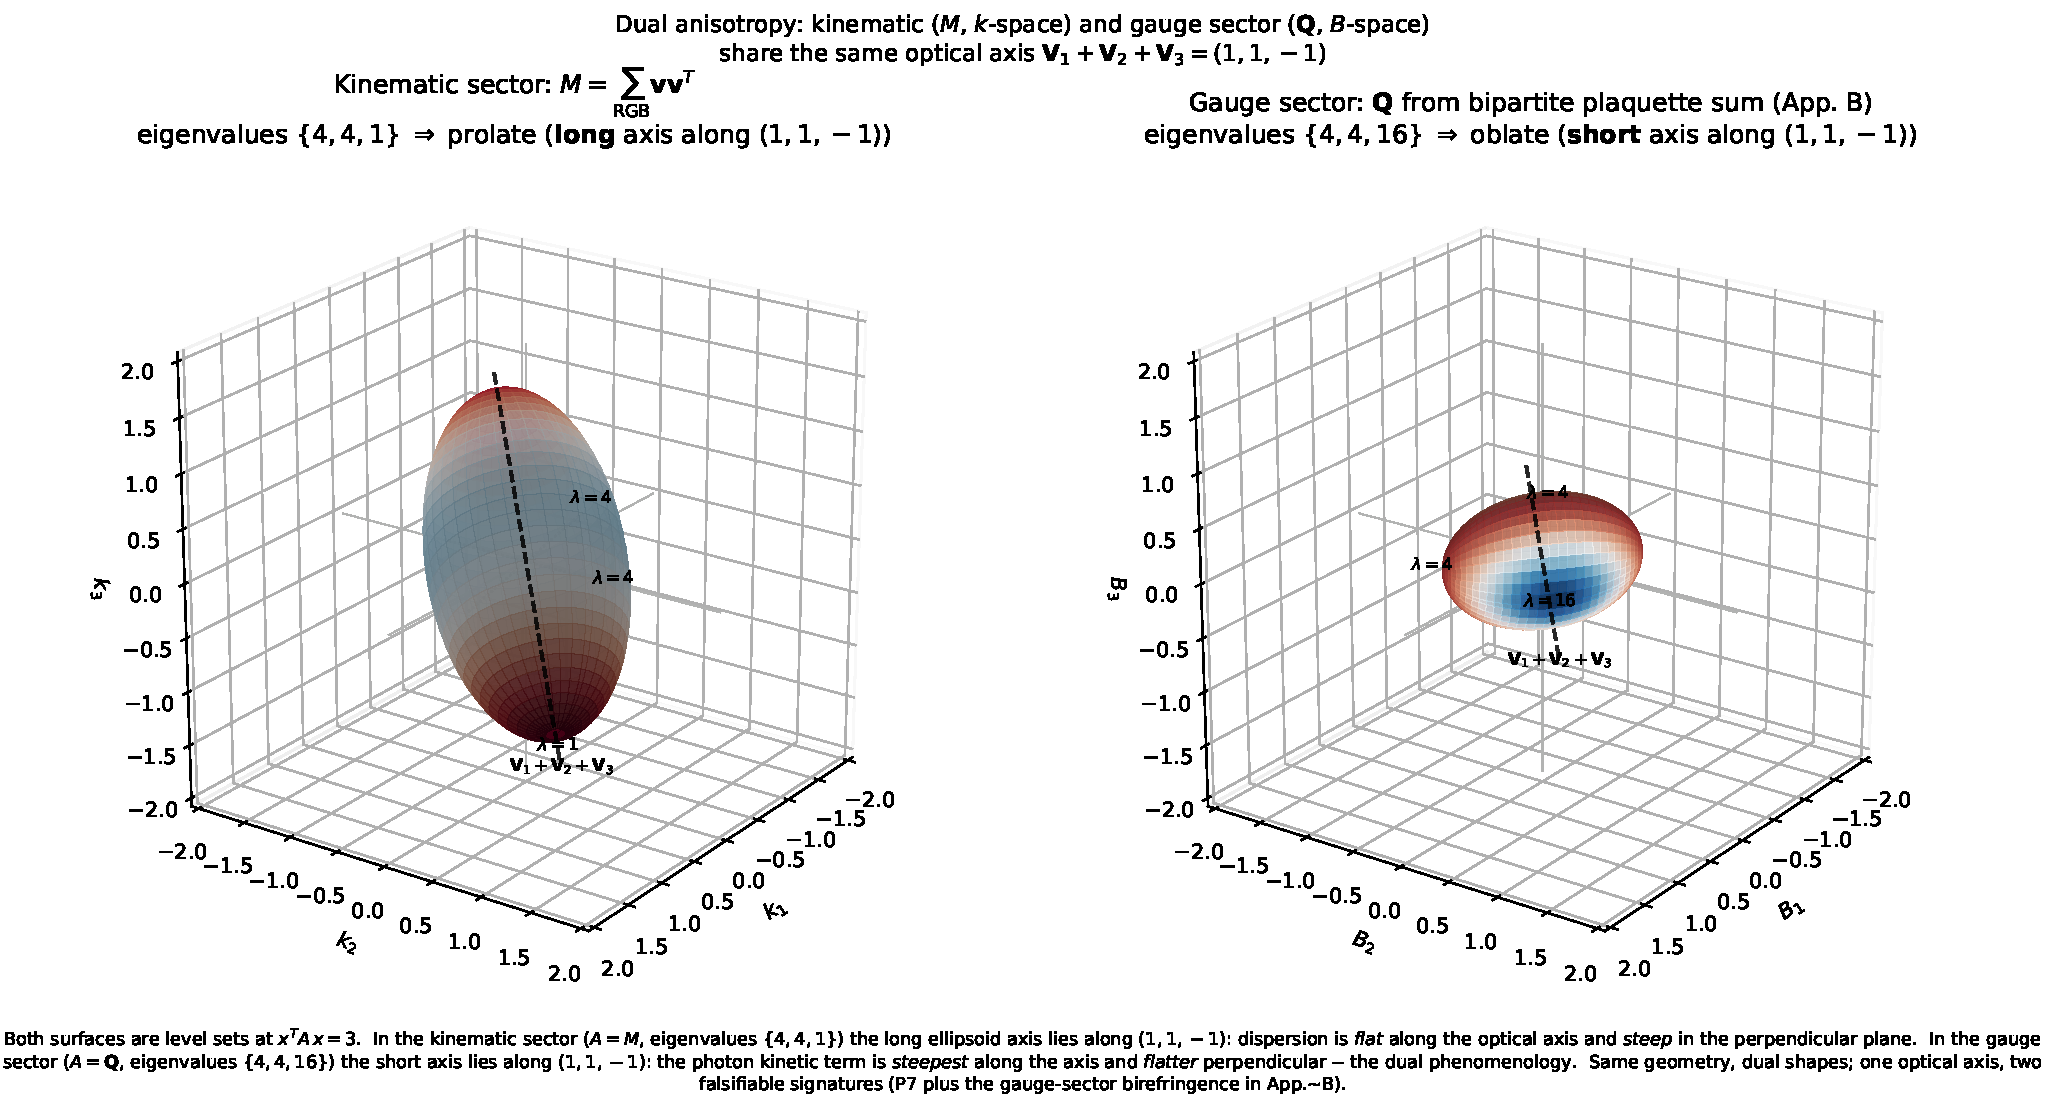
\includegraphics[width=\textwidth]{../figures/induced_action_ellipsoid}
\caption{Dual anisotropy on a single optical axis.
Both panels render level sets at $x^T A\,x = 3$ for the framework's two
anisotropy tensors; both share the special direction
$\mathbf{V}_1+\mathbf{V}_2+\mathbf{V}_3 = (1,1,-1)$ (dashed black line).
\textbf{Left (kinematic sector):} the frame matrix
$M = \sum_\mathrm{RGB}\mathbf{v}\mathbf{v}^T$
(Eq.~\ref{eq:frame_matrix}) on $\mathbf{k}$-space.  Eigenvalues
$\{4, 4, 1\}$ produce a \emph{prolate} ellipsoid whose \emph{long} axis
lies along the optical axis: kinematic dispersion is flat along
$(1,1,-1)$ and steep in the perpendicular plane.  This is the same
quadratic form that underlies the $|\tilde{H}_\text{RGB}|^2$ expansion
of $M_\text{eff}$ (Eq.~\ref{eq:M_eff},
Section~\ref{subsec:p7_photon_dispersion}).
\textbf{Right (gauge sector):} the bipartite plaquette tensor
$\mathbf{Q}$ (Eq.~\ref{eq:Q_matrix}) on $\mathbf{B}$-space (the Hodge
dual of antisymmetric $F_{ij}$).  Eigenvalues $\{4, 4, 16\}$ produce an
\emph{oblate} ellipsoid whose \emph{short} axis lies along $(1,1,-1)$:
the induced photon kinetic term is steepest along the optical axis and
flatter perpendicular --- the dual of the kinematic shape.  Both
anisotropies inherit the special direction from the same bipartite
RGB/CMY geometry; the dual ellipsoid shapes give two independent
falsifiable signatures with one optical axis (kinematic-sector birefringence
in P7, gauge-sector birefringence in Appendix~\ref{sec:induced_gauge_action}).}
\label{fig:induced_action_ellipsoid}

\end{figure}

% ── B.5 O_h averaging recovers Maxwell ──────────────────────────────────────
\subsection{$O_h$ averaging recovers Maxwell}
\label{subsec:induced_maxwell}

Physical observables on the lattice must be invariant under the
crystallographic point group $O_h$ (order 48), which acts
simultaneously on the spatial coordinates and on the antisymmetric
$\mathbf{F}$-space.  Averaging
Eq.~\eqref{eq:plaquette_sum_quadratic} over $O_h$ gives
\begin{equation}
    \bigl\langle\,\mathbf{F}^{\!T}\,\mathbf{Q}\,\mathbf{F}\,\bigr\rangle_{O_h}
        = \frac{\mathrm{Tr}\,\mathbf{Q}}{3}\,
            \sum_{i<j} F_{ij}^2
        = 8\,\sum_{i<j} F_{ij}^2.
    \label{eq:Oh_averaged}
\end{equation}
Using $F_{\mu\nu} F^{\mu\nu} = 2\sum_{i<j}F_{ij}^2 + (\text{electric
contribution})$ and absorbing the
$\sum_{i<j} F_{ij}^2 \to \tfrac{1}{2}F_{\mu\nu}F^{\mu\nu}$
identification in the magnetic sector, the leading $O_h$-averaged
induced action is
\begin{equation}
    S_\text{eff}^{(\text{leading})}[A]
        \;\xrightarrow[a\to 0]{O_h\text{ average}}\;
        \frac{2 c}{3}\int d^4x\;
            \tfrac{1}{2}F_{\mu\nu}(x)\,F^{\mu\nu}(x),
    \label{eq:Maxwell_recovered}
\end{equation}
the standard Maxwell action.  The numerical prefactor $c = 1/g^2$
remains to be determined by the explicit one-loop
$-\mathrm{Tr}\,\ln D_\text{lat}[U]$ calculation; what is determined
here is that whatever prefactor that calculation produces, the
$O_h$-averaged form of the leading induced term is the standard
Maxwell density.

The pre-averaging operator-level density carries the residual
\begin{equation}
    S_\text{eff}^{(\text{operator})}[A]
        = S_\text{eff}^{(\text{leading})}[A]
        + \frac{c\,a^4}{2}\,\mathbf{F}^{\!T}\,\mathbf{Q}_\text{aniso}\,\mathbf{F}.
    \label{eq:operator_residual}
\end{equation}
The $\mathbf{Q}_\text{aniso}$ term is the gauge-sector birefringence:
a closed-form, direction-dependent contribution to the photon
dispersion with optical axis $(1,1,-1)$.  It is the gauge-field
twin of the kinematic prediction of
Section~\ref{subsec:p7_photon_dispersion}.

% ── B.6 Status: structural step closed, numerical prefactor open ────────────
\subsection{Status of the induced-action programme}
\label{subsec:induced_status}

The structural step of the programme set out in
Section~\ref{subsec:open_program} is closed by this appendix:

\begin{itemize}
\item \textbf{Locality + gauge invariance + minimality} force the
    leading-order induced action to be quadratic in $F_{ij}$,
    summed over closed plaquette holonomies
    (Section~\ref{subsec:induced_plaquette_sum}).
\item \textbf{The bipartite RGB/CMY geometry} fixes the tensor
    coefficient $\mathbf{Q}$ with eigenvalues $\{4, 4, 16\}$
    (Section~\ref{subsec:induced_birefringence}).
\item \textbf{$O_h$ averaging} recovers the standard Maxwell density
    up to the numerical prefactor $c = 1/g^2$
    (Section~\ref{subsec:induced_maxwell}).
\item \textbf{The operator-level residual} is a closed-form
    anisotropic tensor whose special direction matches the
    kinematic-sector optical axis $(1,1,-1)$
    (Eq.~\ref{eq:operator_residual}).
\end{itemize}

What remains to fully close the programme is the explicit numerical
calculation of $c = 1/g^2$.  This is a one-loop lattice perturbation
theory calculation for the bipartite Dirac operator
$D_\text{lat}[U]$.  Standard staggered-fermion machinery
(Kogut--Susskind, Susskind 1977; cf.~Section~\ref{subsec:dirac_limit})
applies, with the doubler structure and the bipartite RGB/CMY
chirality projection requiring careful bookkeeping.  We flag this as
a paper-length follow-on project.  The numerical $1/g^2$ prefactor is
the only remaining open item in the induced-action programme: the
structural form, the bipartite $\mathbf{Q}$-tensor with eigenvalues
$\{4, 4, 16\}$, and the closed-form gauge-sector birefringence along
the $(1,1,-1)$ optical axis are all in hand.

The structural form, including the prediction of gauge-sector
birefringence with optical axis $(1,1,-1)$, is established
independently of that calculation.  This converts the asymmetry
flagged in Section~\ref{subsec:honest_scope} -- gravity end-to-end
versus electromagnetism postulating the Wilson action -- into a
narrower asymmetry: gravity is fully derived; electromagnetism is
derived up to a numerical coupling constant.  The induced action
itself, with its leading structural form and bipartite anisotropy,
is no longer a postulate.

% ── B.7 Reproducibility ─────────────────────────────────────────────────────
\subsection{Reproducibility}
\label{subsec:induced_reproducibility}

The full symbolic calculation is performed in
\texttt{src/utilities/induced\_gauge\_action.py}.  Running
\begin{verbatim}
    python -u src/utilities/induced_gauge_action.py
\end{verbatim}
reproduces every numerical claim in this appendix and writes the
captured output to \texttt{data/induced\_gauge\_action.txt}.  The
calculation requires only \texttt{sympy}; no specialised lattice
gauge theory infrastructure.

The five-line core verification of $\mathbf{Q}$'s eigenvalues is
\begin{verbatim}
    import sympy as sp
    V1, V2, V3 = sp.Matrix([1,1,1]), sp.Matrix([1,-1,-1]), sp.Matrix([-1,1,-1])
    F = sp.Matrix(3, 3, lambda i,j: sp.Symbol(f"F{i}{j}", real=True)*(1 if i<j else (-1 if i>j else 0)))
    proj = lambda Va, Vb: sum(Va[i]*Vb[j]*F[i,j] for i in range(3) for j in range(3))
    Q_density = sum(sp.expand(proj(V,W)**2) for V,W in [(V1,V2),(V1,V3),(V2,V3)])
\end{verbatim}
extracting $\mathbf{Q}$ from the quadratic form in the $\{F_{12},F_{13},F_{23}\}$
basis yields Eq.~\eqref{eq:Q_matrix} and the eigenvalues
$\{4, 4, 16\}$.


\section{Reproducibility Quickstart}
% ============================================================
% reproducibility.tex
% Appendix C: Reproducibility Quickstart
% ============================================================

\label{sec:reproducibility}

This compact appendix lets a reviewer verify a working build of the
numerical machinery in under a minute, without reading
Appendix~\ref{sec:code_and_data}'s full technical detail.  All paths
and commands assume the repository root as the working directory.

\subsection*{C.1 Snapshot}

\begin{itemize}\setlength{\itemsep}{0.2em}
\item \textbf{Repository:}
\href{https://github.com/JackDMenendez/discrete-causal-lattice}%
{\texttt{github.com/JackDMenendez/discrete-causal-lattice}}
\item \textbf{Tag for this paper:} \texttt{v0.98-RC}
\item \textbf{Zenodo DOI:}
\href{https://doi.org/10.5281/zenodo.20017133}%
{\texttt{10.5281/zenodo.20017133}}
(commit hash recorded in the Zenodo deposit metadata)
\item \textbf{License:} MIT
\item \textbf{Contact:} \texttt{jackdmenendez@gmail.com}
\end{itemize}

\subsection*{C.2 Minimum environment}

\begin{itemize}\setlength{\itemsep}{0.2em}
\item Python~3.14.4, \texttt{numpy~2.4.3}, \texttt{scipy~1.17.1}
\item Tested on Windows~11 (MSYS2 UCRT64) and Linux
\item No GPU; consumer-grade CPU sufficient
\item Full pinned dependencies and toolchain notes in
Appendix~\ref{sec:code_and_data}
\end{itemize}

\subsection*{C.3 Hardware and observed runtimes}

Wall-clock times measured during preparation of this paper on a
single consumer CPU (8-core, 16-thread, no GPU acceleration):

\begin{itemize}\setlength{\itemsep}{0.2em}
\item \texttt{exp\_12b} smoke test (TICKS=20, 65$^3$ grid): $\sim 14$ s.
\item \texttt{exp\_12b} full baseline (TICKS=6000, 65$^3$ grid):
$\sim 87$ min, single worker.
\item \texttt{exp\_20} three-arm full sweep (TICKS=6000 per arm,
65$^3$ grid): $\sim 119$ min wall-clock with three parallel workers.
\item \texttt{exp\_19c} v10 sweep (TICKS=6000 per rate, 65$^3$ grid,
five rates): $\sim 5$~h per worker, five parallel workers.
\end{itemize}

\subsection*{C.4 Three canonical entry points}

The three experiments most directly load-bearing for the audit-table
claims are runnable with single commands.  In each case
\texttt{TICKS=20} is the smoke-test mode (verifies the wiring in
seconds); the production runs reproduce the full numbers cited in
the paper.

\begin{quote}\small\ttfamily
\# Two-body Bohr radius (k\_min = 0.0970 vs k\_Bohr = 0.0971)\\
make -C src/experiments exp\_12\\[0.5em]
\# Three-arm emission operator comparison (joint A=1 verification)\\
EXP20\_TICKS=6000 python src/experiments/\\
\hphantom{xxxx}exp\_20\_emission\_operator.py\\[0.5em]
\# Long-duration two-body baseline (no emission)\\
EXP12B\_TICKS=6000 python src/experiments/\\
\hphantom{xxxx}exp\_12b\_twobody\_long\_baseline.py
\end{quote}

\subsection*{C.5 Minimal verification snippet}

The fastest end-to-end check.  Runs \texttt{exp\_12b} for 20 ticks
(approximately 14~s on the reference hardware) and prints two
scalars that a clean checkout must reproduce.

\begin{quote}\small\ttfamily
\# verify\_install.py --- run from repository root\\
import os, subprocess, numpy as np\\
os.environ['EXP12B\_TICKS'] = '20'\\
subprocess.check\_call([\\
\hphantom{xx}'python', 'src/experiments/exp\_12b\_twobody\_long\_baseline.py'\\
])\\[0.3em]
arr = np.load('data/exp\_12b\_baseline.npy')\\
\# index layout: [settled, max\_streak, T\_settle, amp\_e, amp\_p,\\
\#                A\_drift\_max, rho\_drift\_max, r\_peak\_min, r\_peak\_max]\\
r\_peak\_min = arr[7]; A\_drift = arr[5]\\
print(f"r\_peak\_min = \{r\_peak\_min:.3f\}\hphantom{x}expected $\approx$ 9.877")\\
print(f"A\_drift\hphantom{xxxxx} = \{A\_drift:.2e\}\hphantom{xx}expected $\approx$ 4.4e-16")
\end{quote}

\noindent\textbf{Reference output} (bit-exact on the reference
software stack; deterministic by construction --- the framework
uses no RNG for any of these three experiments):

\begin{quote}\small\ttfamily
r\_peak\_min = 9.877\hphantom{x}expected $\approx$ 9.877\\
A\_drift\hphantom{xxxxx} = 4.44e-16\hphantom{x}expected $\approx$ 4.4e-16
\end{quote}

If both scalars match within $\sim 1\%$ of the reference values, the
numerical machinery reproduces.  $\mathcal{A}$-drift at machine
precision ($\lesssim 10^{-15}$) is the structural correctness check:
the bipartite tick rule preserves $\sum_i \lVert\psi_i\rVert^2$
exactly under \texttt{tick(normalize=True)}, so any larger drift
indicates an environment problem (numerical-precision flag,
incompatible \texttt{numpy} build, etc.).

\subsection*{C.6 If the snippet fails}

\begin{itemize}\setlength{\itemsep}{0.2em}
\item \textbf{\texttt{r\_peak\_min} differs by more than $\sim 5\%$:}
verify the Coulomb constants (\texttt{STRENGTH=30.0},
\texttt{SOFTENING=0.5}) and that
\texttt{src/experiments/exp\_12b\_twobody\_long\_baseline.py}
imports a clean \texttt{src/core} module set; a stale
\texttt{\_\_pycache\_\_/} can also matter.
\item \textbf{\texttt{A\_drift} larger than $\sim 10^{-12}$:}
indicates a different floating-point environment than the reference
stack; check \texttt{numpy} build flags and BLAS backend.
\item \textbf{Import error / module not found:} re-run \texttt{make
env} or check that the project virtualenv is activated; the script
imports \texttt{src.core.\{OctahedralLattice, CausalSession,
enforce\_unity\_spinor\}}.
\item For full troubleshooting, see Appendix~\ref{sec:code_and_data}.
\end{itemize}

\subsection*{C.7 Beyond the smoke test}

The full audit-table evidence cited in this paper requires the
production runs in §C.4, not the 20-tick smoke test.  Wall-clock
budgets are given in §C.3.  Each experiment writes its own
\texttt{.log} (per-window progress) and \texttt{.npy} (summary array)
under \texttt{data/}; the per-experiment documentation in
\texttt{src/experiments/*.md} states the expected results, runtime,
and any non-default flags.


%% ============================================================
\bibliographystyle{unsrt}
\bibliography{paper-bib/references}

\end{document}
